\documentclass[10pt,a4paper]{article}
\usepackage[utf8]{inputenc}
\usepackage{amsmath}
\usepackage{amsfonts}
\usepackage{amssymb}
\usepackage{relsize}
\usepackage{blindtext}
\usepackage{tcolorbox}
\usepackage{graphicx}
\usepackage{hyperref}
\usepackage{pdfpages}

\graphicspath{ {./images/} }

\title{Twitter User Localization\\[0.2em]\smaller{Master Thesis Report}}
\author{Silas Berger}

\makeindex

\begin{document}

\maketitle
\clearpage

\section*{Abstract}
Knowing a social media user's location can be useful for many applications in data analysis, in fields such as market research, public health, and politics. Researchers often use Twitter as their platform of choice for this type of analysis, as it provides a vast repository of publicly available data. Unfortunately, many Twitter users choose not to disclose their true location. Many research projects have investigated ways of accurately estimating a Twitter user's location withing a given radius (e.g. 10km). Since this has proven to be a considerable challenge, we have decided to simplify the problem to a binary classification between Swiss and non-Swiss (i.e. foreign). This information can often be just as useful as localizing a Twitter user to a city or precise location, especially in a small country such as Switzerland. Therefore, sacrificing some specificity in this localization may be a worthwhile trade-off, if it allows for more reliable results.

Since we were unable to find an existing Twitter-based data set which fit our needs for this project, we built a custom data set, specifically oriented towards our research. This data set is based around a collection of Twitter users we refer to as "Swiss Influencers" - that is, accounts which are mostly of interest to Swiss people. We then defined a set of features considered likely to be indicators as to whether a certain Twitter user is Swiss or foreign. We implemented these features as part of a full classification pipeline which allows users to specify the screen name of a Twitter user and receive as a result a classification of that Twitter user as either Swiss or foreign. 

We have found that our best classification models achieved an accuracy of 95\%, with a maximum precision of 98\%, and a maximum recall of 91\%. To the best of our knowledge, research projects attempting to localize Twitter users to a precise radius (e.g. 10km) managed to correctly localize at most 60\% of users. This goes to show that our binary classification problem, while potentially not being specific enough for certain types of applications, can amount to significantly more reliable results.

\clearpage
\tableofcontents
\clearpage

\section{Introduction}
Knowing a social media user's location can be useful for a variety of applications in areas such as public health, public safety, or sales. This type of research is often done using Twitter. Twitter users have the option to specify their location on their profile page. However, many users choose not to do so, or supply a made-up location value. We therefore want to explore ways to localize a Twitter user based on their data accessible to us through the Twitter API, even if they do not supply a valid location field.

For this, we have compiled a list of "Swiss Influencers" - that is, a list of Twitter accounts which are likely mostly followed by Swiss users. These influencers include accounts such as local sports teams, local politicians, and other public which are mostly of interest to Swiss people, such as Swiss TV stations and newspapers. If such a Swiss public figure or entity is also well-know outside of the country, it is not considered a Swiss Influencer. For example, this is true for public figures such as Roger Federer. While he is Swiss, he also has fans around the world, which means his Twitter account will likely be followed by many people outside of Switzerland. Since we were unable to find any existing Twitter data sets suitable for our purposes, we then created our own database of Twitter users and their Tweets.

We propose a number of features which can be used as indicators to determine whether a given Twitter user is Swiss or foreign. We have developed a full pipeline for localizing Twitter users through a web front end.

\section{Goals}
We want to build a data set of Twitter users, starting with a set of users we have determined to be “Swiss Influencers” (that is, popular users which are likely mostly followed by Swiss people), and the users who follow them. We want to augment the information in this dataset by collecting recent Tweets of as many of these users as possible.

We want to analyze these data, to answer the following research question:

\begin{tcolorbox}[width=\textwidth,colback={white},title={RQ},arc=0mm,outer arc=0mm,colupper=black]    
    \textit{Can we use this information to reliably determine whether or not a certain Twitter user is Swiss?}    
\end{tcolorbox}  

A Twitter user's classification into Swiss or non-Swiss will necessarily introduce some amount of uncertainty. It would be useful to know how reliable a given classification is. We therefore want to accompany each classification with a value that conveys the confidence in that classification. However, since the focus of this project lies on investigating ways to localize users and on building a data set and a complete localization pipeline, we will limit ourselves to using the most common approach of confidence estimation, as outlined in our related work section.

In order to give users of our system a way of interacting with the data and the localization metamodels, we also want to implement a RESTful interface. This API should allow them to retrieve basic statistics about the collected data and the localization metamodels in use, such as the percentage of users classified as Swiss and non-Swiss respectively, the average confidence of a given meta-model, as well as the average precision and recall of a given meta-model. Furthermore, the API should provide a way for users to supply a new Twitter user object to the system, to classify that user as Swiss or non-Swiss. 

Finally, we want to implement a simple web-based user interface to provide a graphical way of interacting with the API. The web interface should allow users to study graphical representations of the data at hand, to help them better understand the data and the localization metamodels. Users should also be able to localize a new Twitter user using the web interface.

\section{Related Work}
Related research shows that only a small number of users indicate a valid and precise location in their profile's location field. Roughly 28 to 34\% of Twitter users do not indicate a location at all, while many of the others provide a nonsensical value such as \textit{Wonderland} or \textit{Worldwide}, or an unspecific location such as \textit{California} \cite{chen10a, hech11a}. This underlines the strong potential of estimating a user's location \cite{chen10a}, with applications in areas such as earthquake detection \cite{robi11a, saka10a} (figure \ref{fig:earthquake-center-estimation}), typhoon trajectory estimation \cite{saka10a} (figure \ref{fig:typhoon-trajectory-estimation}) and the prediction of emerging influenza epidemics \cite{achr11a}.

\begin{figure}
	\centering
	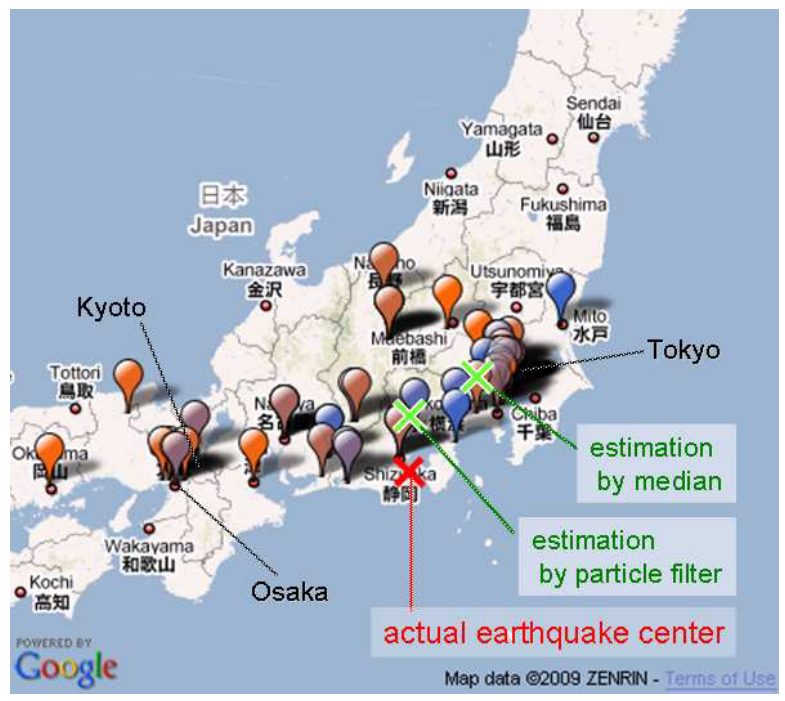
\includegraphics[scale=0.60]{earthquake-center-estimation}
	\caption{Earthquake center estimation using Twitter data \cite{saka10a}}
	\label{fig:earthquake-center-estimation}
\end{figure}

\begin{figure}
	\centering
	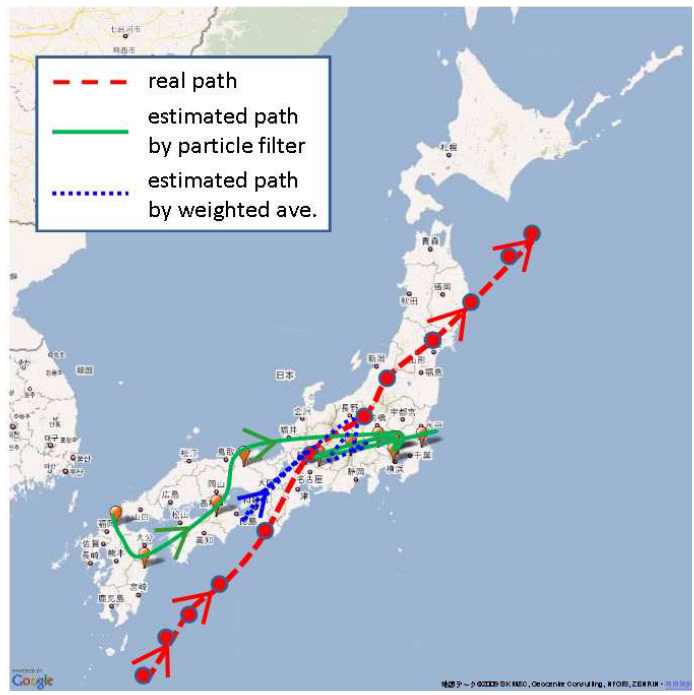
\includegraphics[scale=0.60]{typhoon-trajectory-estimation}
	\caption{Typhoon trajectory estimation using Twitter data \cite{saka10a}}
	\label{fig:typhoon-trajectory-estimation}
\end{figure}

As a ground truth for their localization models, researchers tend to utilize a Twitter user's location field. To verify the user-supplied values, they are matched against a reference database such as Yahoo's geo-localization API, a geographical gazetteer, or against the corresponding Wikipedia page \cite{gonz11a, hech11a, mahm14a}. As an alternative to this user-supplied value, Ryoo et al. (2014) proposed using GPS-tags in a user's Tweets. However, in their data collection, only 0.4\% of all users had GPS-tagging activated \cite{ryoo14a}. In addition to the heavily limited availability of GPS data, this approach also faces the issue that it generally associates a user with multiple locations. This is is however somewhat mitigated by the fact that most Tweets are published either from a user's home or their workplace \cite{ryoo14a}.

\begin{figure}
	\centering
	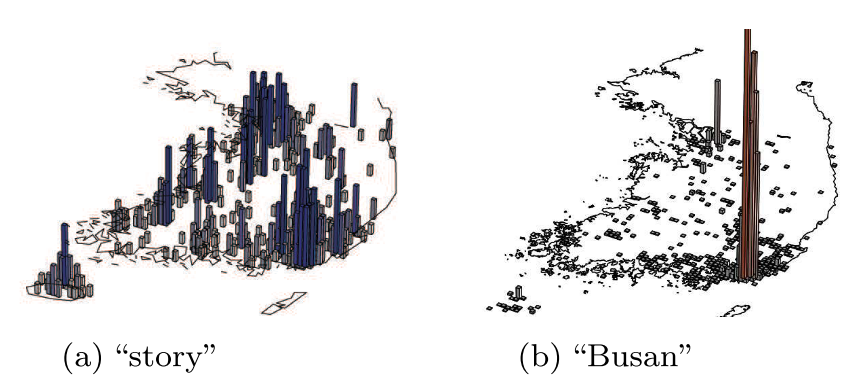
\includegraphics[scale=0.60]{spatial-locality-of-words}
	\caption{Demonstration of the spatial locality of the words "story" and "Busan" in South Korean Tweets \cite{ryoo14a}}
	\label{fig:spatial-locality-of-words}
\end{figure}

\begin{figure}
	\centering
	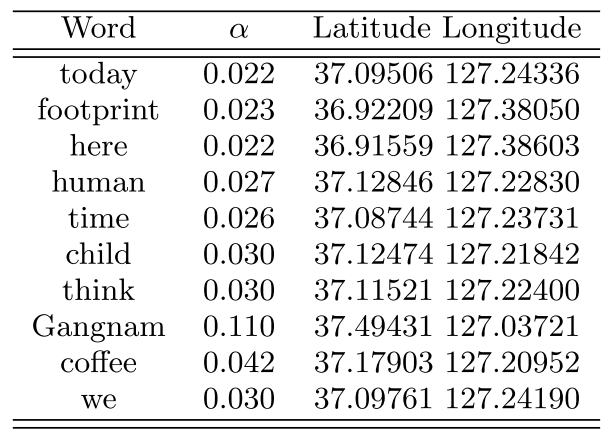
\includegraphics[scale=0.60]{alpha-values-of-frequent-words}
	\caption{$\alpha$ values of the most frequent words in their dataset \cite{ryoo14a}}
	\label{fig:alpha-values-of-frequent-words}
\end{figure}

\begin{figure}
	\centering
	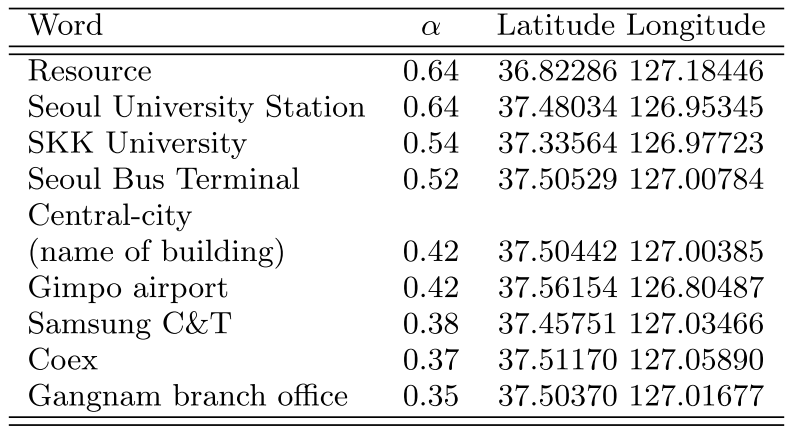
\includegraphics[scale=0.60]{words-with-high-alpha-value}
	\caption{Words with high $\alpha$ values \cite{ryoo14a}}
	\label{fig:words-with-high-alpha-value}
\end{figure}

Most localization approaches so far rely on users' Tweet contents and Tweet behaviour \cite{ryoo14a, chen10a, hech11a, chi14a, mahm14a, chan12a, han16a}. Ryoo et al. (2014) \cite{ryoo14a} proposes the use of a probabilistic model to infer a user's main location of activity on Twitter using their textual contents. As a central component of their model, they use the spatial locality of select words, as demonstrated in figure \ref{fig:spatial-locality-of-words}. The researchers quantify this locality quality in a value referred to as \textit{$\alpha$ value}. Figure \ref{fig:alpha-values-of-frequent-words} shows the $\alpha$ values of the most frequent words in their dataset. Figure \ref{fig:words-with-high-alpha-value} gives an overview of selected words with a high spatial locality, that is, a high $\alpha$ value. This approach enables them to locate 60\% of Korean Twitter users within 10km of their location. A similar approach was proposed by Cheng et al. (2010), who use a maximum likelihood model based on word frequencies in Tweets from a given city \cite{chen10a}. Their model is able to place 51\% of their tested Twitter users within 100 miles of their correct location.

Such approaches require a method to avoid noise words. That is, for every word seen in a user's Tweets, it is necessary to decide whether that word conveys a strong sense of location. For instance, the word \textit{howdy} is a typical greeting in Texas, while other words such as \textit{august}, \textit{peace} and \textit{world} to not convey a strong sense of location \cite{chen10a}.

In contrast to these approaches, Compton et al. (2014) proposes using the locations of a Twitter user's friends \cite{comp14a} (that is, accounts followed by this user) to estimate the user's location. Rodrigues et al. (2013) proposes the use two sources of information: the user's Tweets and their friendship network \cite{rodr13a}. As additional data sources, researchers use features such as timezone values, or a one-hot bag-of-words vector representation of a user's self-description (i.e. "biography") \cite{han16a}. Further approaches proposed the use of a user's dialect, their interaction with local issues such as sports teams, and their Twitter conversations, in the form of Reply-Tweets. \cite{dred13a, chan11a}. 

As an additional source of data, it may also be useful to link a Twitter user to their profiles on other social media platforms, such as LinkedIn. However, this can be challenging, due to sparse information and duplicate screen names. Approaches have been proposed to match users across various social media platforms using their life events such as graduation, marriage or new job, as well as their profile biographies \cite{hazi17a}.

\begin{figure}
	\centering
	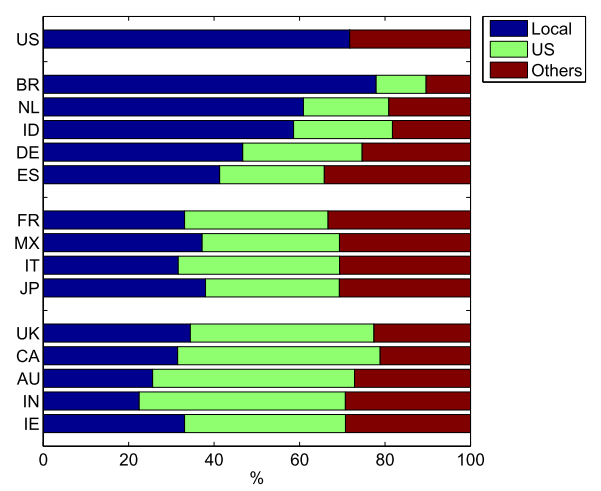
\includegraphics[scale=0.80]{follower-distribution}
	\caption{Percentage of followers within the country, in US and in other countries \cite{gonz11a}}
	\label{fig:follower-distribution}
\end{figure}

Gonzalez et al. (2011) demonstrated that countries in countries with English as an official language or co-language usually have more followers in the US than within their same country. In contrast, users in countries with different languages, such as Brazil, tend to have the majority of their followers in their own country. A potential reason for this effect is the fact that the US are a dominant country on Twitter, accounting for around half of the total number of users worldwide (2011) \cite{gonz11a}. This effect is outlined in figure \ref{fig:follower-distribution}.

For our research, we require a dataset of Twitter users with known location, as well as their Tweets. To the best of our knowledge, none of the publicly available datasets are suitable for our purpose. We will therefore have to create our own custom dataset of Twitter users and Tweets for our purpose. As outlined by van der Veen (2015) \cite{vand15a}, a useful approach to this task is to define a set of keywords, which can then be sent to the Twitter API as queries for Tweets.

For our project, we need to handle large quantities of heterogenous data without introducing too much delay on queries. The canonical approach for storing for many years has been using relational database management systems (RBMS), such as MySQL \cite{mysq15a} or PostgreSQL \cite{ston95a},because of their performance and data integrity guarantees. However, as Győrödi et al. (2015) \cite{gyor15a} mentions, NoSQL alternatives such as MongoDB offer more flexibility for heterogenous data, which is important for our application. As also pointed out by Győrödi et al. (2015) \cite{gyor15a}, a benefit of choosing MongoDB as such an alternative is the fact that it has a large user base, and thus a large community on the forums. 

In addition to storing Twitter user metadata and Tweets, we also require a solution for storing data in a graph format. A modern solution for storing and analyzing such data is presented by graph databases such as Neo4j and ArangoDB \cite{best19a}. As observed by López et al. (2015) \cite{lope15a}, Neo4j tends to show the best performance in terms response times, when compared RDBMS and other graph databases. Aside from this factor, the core differences in the various available graph databases lie in their data model and features, as analyzed by Fernandes and Bernardino (2018) \cite{fern18a}.

Finally, we want to accompany each Swiss / non-Swiss classification with a value that conveys the classifiers confidence in its decisions. As pointed out by Devarakota et al. (2007) \cite{deva07a}, this can be especially relevant for security-sensitive applications, as a way to reject samples with a high chance of false classification. As also observed by Devarakota et al. (2007) \cite{deva07a}, the most common approach to this is to use the estimated class membership probability of each classifier to serve as a prediction confidence value. However, both Devarakota et al. (2007) \cite{deva07a} and Alasalmi et al. (2016) \cite{alsa16a} also propose more complex approaches to this problem, which can result in more reliable confidence estimates.

In summary, we see that there are two main groups of approaches to localizing a Twitter user. Researchers either use the textual contents of a Twitter user's Tweets or self-description, or the use aspects of their friendship network, such as their follows-relationships and their retweet and reply-tweet behavior. In the former approach, researchers often look for specific words that can be considered indicators of a user's location, such as words with strong spatial locality \cite{ryoo14a}. Approaches relying on textual content generally have a few challenges in common, such as having to deal with noisy data, and having to adapt models to different languages. Additionally, users may not always adhere to proper grammar and orthography when posting on social media, making Natural Language Processing tasks even more difficult. That said, noisy data is also an issue when taking the approach of examining a user's friendship and interaction network. Some accounts may be oriented towards maximizing exposure and thus follow and interact with an exceptionally large number of other users. Another source of noise in this approach is the circumstance that users may choose to (partially) ignore accounts from within their region or country, in favor of following accounts that are relevant with respect to their particular interests. For instance, a user with an interest in computer science may favor accounts by relevant people in that field, such as Elon Musk (Tesla Motors / SpaceX), Sundar Pichai (Google) or Bill Gates (Microsoft), rather than those of their region's local media outlets, politicians, or friends living in the region. This goes to show that both of these groups of approaches may work well for some given Twitter user, but can fail for another. Whether an approach is successful largely depends on what assumptions it needs to make, and whether a given Twitter user in question fulfills them.

\section{Design}
We break our classification system down into three core components: features, classifiers, and metamodels.

\subsection{Features}
In our architecture, we define a feature extractor as an algorithm that analyzes our database or graph, to produce a scalar or vector describing a pivot user in terms of some defined property. We call this resulting scalar or vector a “feature”. We propose the following features:
\begin{itemize}
\item \textbf{Influencer Follower Ratio:} The number of Swiss Influencers a given user follows, divided by the total number of accounts followed by this user.
\item \textbf{Swiss Tweet Interactions Ratio:} The proportion of a given user's Tweets that interact with interact with accounts known to be Swiss, via the use of @mentions, Retweets, and Tweet replies. The more a user interacts with Swiss Twitter users, the more likely they may be to be Swiss themselves.
\item \textbf{Tweet Interactions Behavior:} The proportion of all @mentions, Retweets, and Tweet replies per Tweet, in a given user's Tweets. Swiss- and non-Swiss users may show different patterns in their overall Tweet interaction behavior.
\item \textbf{Hashtag Similarity:} The relative size of the overlap between a user's $n$ most frequently used hashtags and the $n$ most frequently used hashtags among all Swiss users in the training set. Hashtags indicate which topics a user is Tweeting about, and these topics may be similar among Swiss users.
\item \textbf{NER Swiss Places} The number of recognized Named Entities in a user's Tweets that refer to a populated place in Switzerland. The more such places a user mentions, the more likely they may be to be Swiss.
\item \textbf{NER Similarity} The relative size of the overlap between a user's $n$ most frequently mentioned Named Entities and the $n$ most frequently used Named Entities among all Swiss users in the training set.The relative size of the overlap between a user's $n$ most frequently used hashtags and the $n$ most frequently used hashtags among all Swiss users in the training set. Similar to hashtags, Named Entities may indicated the topics a user is Tweeting about, which may be similar among Swiss users.
\item \textbf{Social Media Connection} Try to match a user's Twitter profile to their presence on other social media such as LinkedIn\footnote{\href{https://www.linkedin.com/}{https://www.linkedin.com/}} and XING\footnote{\href{https://www.xing.com/}{https://www.xing.com/}}. On these more professionally oriented platforms, users may be more likely to correctly state their true location. By matching a user's Twitter profile to their accounts on other social media, we might therefore be able to leverage more accurate user-generated data. 
\end{itemize}

\subsection{Classifiers}
Our localization pipeline defines a classifier is an algorithm that takes in a scalar feature or a feature vector, and produces  a binary Swiss- / non-Swiss decision, together with an estimated confidence. Classifiers are not in charge of handling their own feature extraction. Instead, they are provided with the required / desired features by the meta-model. Generally, classifiers are agnostic to the features they accept. However, there may be exceptions, where certain classifiers expect a specific feature or feature vector. Examples of possible classifiers are as follows:
\begin{itemize}
\item Single-Feature Binary Classifier
\item k-Nearest Neighbours
\item Naive Bayes
\item Decision Tree
\item Scalable Vector Classifier
\end{itemize}

\subsection{Metamodels}
A meta-model is what we call an entity that unites features and classifiers. It consists of one or more classifiers and is responsible for providing them with training and validation data. It defines feature extractor and classifier settings, runs feature extractors, trains classifiers, and combines classifier outputs into a single decision if needed. The meta-model adds each of its classification decisions to the graph as a node-edge-pair, where the edge contains attributes such as the classifier, classifier instance, meta-model, meta-model instance, confidence, etc., while the node mainly contains the class decision. If such an edge represents a meta-model instance's final decision for a given pivot user, the edge is marked as "type: final". Metamodels can also use a combination of multiple classifiers. In this case, each edge representing an individual classifier's decision is marked as "type: partial". The edge representing the final meta-decision is then again marked as "type: final".

Each meta-model first needs to be trained, and can then be used to classify new samples. The training phase is handled by the \textit{build()} function, which each meta-model class provides. It is mainly responsible for training the meta-model's classifiers and validating their accuracy.

Multiple metamodels can be active on the graph at the same time, since all modifications to the graph are labeled with the meta-model and meta-model instance.

Metamodels can be as generic or as ad-hoc. For instance, we might have separate metamodels for each relevant scikit-learn classifier, but we might also have a single “Scikit-learn Meta-Model”, which takes a classifier as an option, or even learns the ideal classifier, based on the validation data.

\section{Implementation}
We have discussed our goals and problem statement, as well as the state of the art and our theoretical approach. In this chapter, we will give an overview of the technologies we used, why we chose them, and what the architecture of our localization pipeline looks like. We will also discuss the different data sets we have collected and explain the feature extractors, classifiers and metamodels we have implemented.

\subsection{Architecture and Technologies}
\begin{figure}[!htb]
	\centering
	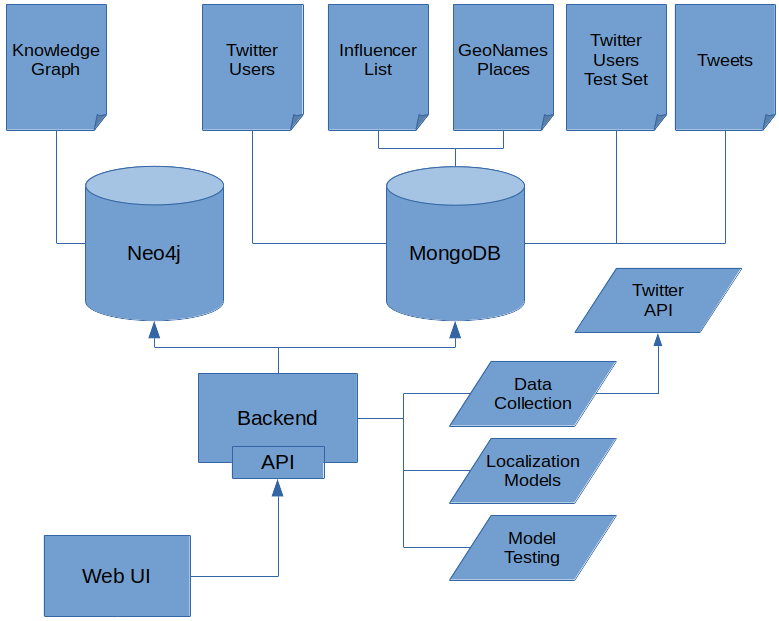
\includegraphics[scale=0.45]{architecture_overview}
	\caption{Architecture Overview}
	\label{fig:architecture-overview}
\end{figure}

Figure \ref{fig:architecture-overview} shows an overview of our software architecture. At the core of our system we have a back end, which is responsible for data collection, localization metamodels, and meta-model testing. The back end uses MongoDB for storing collected data such as Twitter users and Tweets, and Neo4j to build a knowledge graph. It also provides a RESTful API, which is consumed by our web UI.

\subsubsection{MongoDB Database}
We use MongoDB\footnote{\href{https://www.mongodb.com/}{https://www.mongodb.com/}} as our core database system for all data considered mostly static, such as user meta data, user Tweets, and information about geographic locations. We chose MongoDB due to its efficiency, robustness and flexibility in an environment with large amounts of strongly heterogeneous data, as well as its easy-to-use integration with Python. 

Our MongoDB instance is running inside a Docker\footnote{\href{https://www.docker.com/}{https://www.docker.com/}} container, defined by a Docker Compose\footnote{\href{https://docs.docker.com/compose/}{https://docs.docker.com/compose/}} file. This allows for low-cost and low-latency development on any machine, without the need for configuring a database server.

All data is stored in a Docker volume\footnote{\href{https://docs.docker.com/storage/volumes/}{https://docs.docker.com/storage/volumes/}}, where they can be exported to and imported from a TAR file, using a bash script. This is done as a means of creating backups and transferring server states among different development machines.

In our MongoDB database, we maintain the following collections:
\begin{itemize}
\item \textbf{Twitter Users.} Collection of all Twitter user meta data objects we have collected, both influencers and "regular" users. Does not include the users used for testing.
\item \textbf{Influencer List.} Representation of the list of influencers on GitHub\footnote{\href{https://github.com/acknowledge/swiss-twitter-accounts}{https://github.com/acknowledge/swiss-twitter-accounts}}. Storing their screen name, influencer category (politicians, sports teams, media outlets, etc.), and their "fetch status" (i.e. whether we have already fetched the full meta data object for that user). The documents in this collection do not contain the full meta data objects for these users (these are added to the Twitter Users collection and marked as "type: influencer"). This collection currently contains 325 influencer users.
\item \textbf{GeoNames Places.} Meta data object of geographic place specifications corresponding to the GeoNames API. Places are added whenever a user's location field yields a result from the GeoNames API. This collection also contains all PPL*-type\footnote{\href{https://www.geonames.org/export/codes.html}{https://www.geonames.org/export/codes.html}}  GeoNames places for Switzerland, to enable local lookups without being limited by any API rate restrictions.
\item \textbf{Twitter Users Test Set.} A collection of Twitter user meta data objects collected by searching for Tweets matching a list of given keywords. These users are not necessarily related to any of the entries in the Twitter Users collection. All users in this Test Set collection must have a location field that yields a valid result at the GeoNames API, otherwise they are not collected. They all have a GeoNames ID in their user\_place field, which resulted form looking up their location field at the GeoNames API. We use this GeoNames ID as the ground truth for these users' location.
\item \textbf{Tweets.} A collection of Tweets sent out by users in our Test Set collection. 
\item \textbf{Feature Cache.} A collection of documents corresponding to entities in either the Twitter Users or Twitter Users Test Set collection. If a feature extractor extracts a feature value for a given user, that value can be cached in the corresponding document in this collection. This is done as a means to avoid expensive recalculations of feature values.
\end{itemize}

\subsubsection{Knowledge Graph}
We decided to separate our static from our dynamic data, whereby data refers to Twitter user metadata and Tweets gathered from Twitter API, and dynamic data refers to data generated from our metamodels. Since our metamodels generate associations of users and countries, we decided to use a graph database for this part of our implementation. Furthermore, as we are modeling aspects of a social network, we believe that this form of storing our results can offer more flexibility for future expansions than a document store such as MongoDB or an RDBMS. We refer to this graph database as our \textit{knowledge graph}.

As an environment for our knowledge graph, we use the Neo4j\footnote{\href{https://neo4j.com/}{https://neo4j.com/}} graph database. It allows us to easily store and query the relationships among Twitter users, as well as between Twitter users and geographic locations. 

Similar to MongoDB, our Neo4j instance is running inside a Docker container defined by a Docker Compose file, and its data can be exported to and imported from a TAR file.

In the graph, each Twitter user is from the MongoDB database can be depicted as a node. Since all relevant meta data for a user object is already given there, the node only contains core information, such as the user's Twitter ID, which can then be used to get additional data from MongoDB. 

In addition to users, we also have nodes for all geographic locations in Switzerland, provided by GeoNames. Similar to users, these nodes have a reduces set of attributes, in order to save disk space. Since we mostly work with binary classification, the main geographic nodes used are "Switzerland" and "Foreign" - a dummy node representing the location "not Switzerland". This is useful, since classify each user as Swiss or non-Swiss, rather than extracting their explicit country of origin if they are foreign.

When a meta-model localizes a user, it can create an edge in the graph, between that user's node and the location (in our case, "Switzerland" or "Foreign"). The edge can hold attributes such as the meta-model instance by which this localization was created, and the confidence for this decision. This architecture facilitates the process of storing and finding localization decisions made by any meta-model. It also allows different metamodels to persist their partial and final localization decisions simultaneously, without affecting each other. Some use cases include 1) querying for all localization decision made by a specific meta-model instance (useful for evaluating a meta-model's performance), 2) querying for the localization decision made by a specific meta-model for a specific user, and 3) querying for all localization decisions made by any meta-model for a specific user. Figure \ref{fig:knowledge-graph-schema} shows an example of the schema we use for persisting localization results for Twitter users.

\begin{figure}
	\centering
	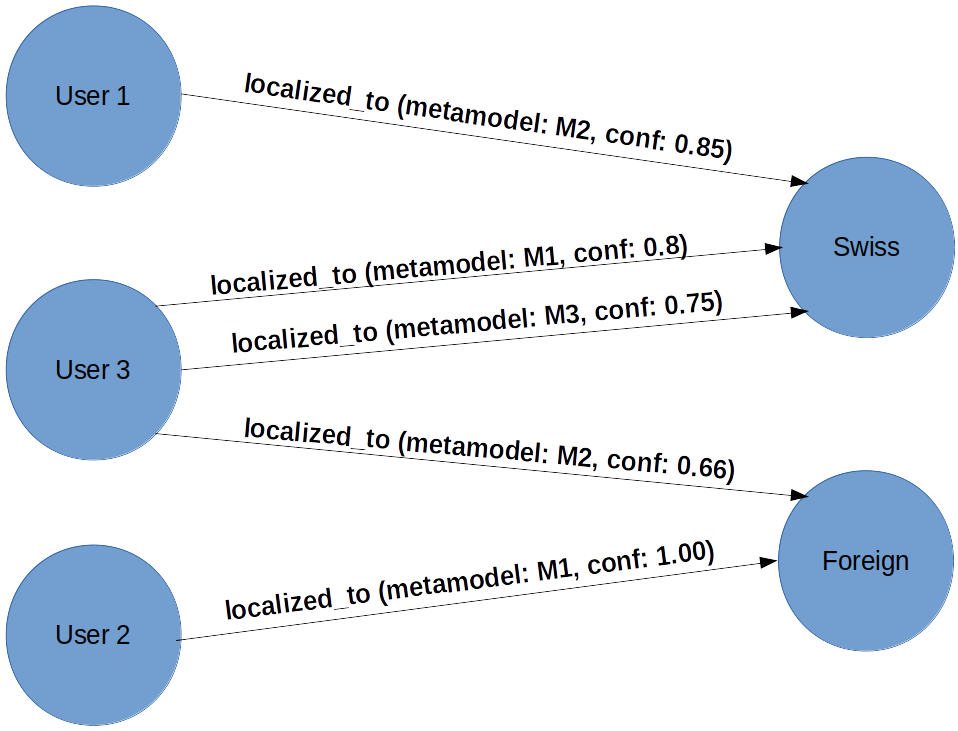
\includegraphics[scale=0.30]{knowledge-graph-schema}
	\caption{Knowledge Graph: Localization Schema}
	\label{fig:knowledge-graph-schema}
\end{figure}

\subsubsection{Tweepy}
We use Tweepy\footnote{\href{https://www.tweepy.org/}{https://www.tweepy.org/}} as a wrapper for interacting with the Twitter REST API. Tweepy offers a seamless integration of API requests and responses into Python code. Additionally, it can automatically await rate limitations and resume its requests afterwards. 

\subsubsection{scikit-learn}
Scikit-learn\footnote{\href{https://scikit-learn.org/stable/}{https://scikit-learn.org/stable/}} is a framework for machine learning in Python. Among other features, it provides implementations for most of the commonly used classifiers, such as k-Nearest Neighbours, Support Vector Machines, Naive Bayes, and Decision Trees, short of Artificial Neural Networks. The provided classifiers are efficient and all use the same interface for training and classification, which makes it easy to switch between different classifiers. This allows us to quickly try out multiple different classifiers in each of our metamodels, in order to find one that works best with the given feature set.

\subsubsection{SpaCy}
For the purpose of Named Entity Recognition (NER), we use SpaCy\footnote{\href{https://spacy.io/}{https://spacy.io/}}, a state-of-the-art framework for Natural Language Processing. NER describes the task of identifying occurrences of a specific object in a sentence, and tagging these objects within a given set of categories. Such categories can include "person", "location", "organization", and so on \cite{lock09a}. We originally intended to use simple PoS tagging using NLTK\footnote{\href{https://www.nltk.org/}{https://www.nltk.org/}}. PoS tagging, as opposed to NER, is the process of marking up each word in a sentence with its specific grammatical part of speech, such as nouns, verbs, adjectives, interjections, and, most importantly for our application, proper nouns. However, NER has proven to be a more useful approach to the problems at hand. Additionally, NLTK does not ship with out-of-the-box PoS tagging support for German, French and Italian. These languages are natively supported by SpaCy, which is another core reason why we decided to use this framework instead.

\subsection{Data Collection}
In order to start building feature extractors and metamodels, we first needed to collect data. As a starting point, we used the already compiled lists of Swiss influencers \footnote{\href{https://github.com/acknowledge/swiss-twitter-accounts}{https://github.com/acknowledge/swiss-twitter-accounts}}. We started by querying the Twitter API for the meta data object for each of the user handles on these lists, and persisting them to the influencers collection in MongoDB. Next, we queried the API for the follower IDs for each of these influencers. This process was rather time-consuming. The Twitter API can be queried for follower IDs a maximum of 15 times per 15-minute window. Additionally, it returns at most 5000 IDs per query. Since our influencers tend to be rather popular accounts, they often have several hundred thousand followers, which means that it can take multiple hours just to retrieve the follower IDs for a single influencer.

After collecting the influencer IDs for all influencers, we proceeded by fetching the meta data objects for all Twitter users corresponding to these IDs. With more than a million distinct IDs and a rate limit of 900 queries per 15-minute window, this again took a long time.

Up to this point, all of our collected Twitter users were either influencers or their followers. In order to get independent sets for training, validation and testing (referred to as the "TVT set"), we developed a crawler that searches the Twitter API for tweets corresponding to a given search term. We defined a list of search terms where some of the terms should yield mostly Tweets by Swiss people, such as "Bundesrat" and "Bundeshaus", while others are not specific to Switzerland, such as "football" and "traffic". Each term was given three times, once in each German, French and Italian, in order to accommodate the three most common official languages in Switzerland. This yielded a total of 15 Swiss-specific terms, and 32 non-specific terms. This list can be found in \hyperref[sec:appendix-searchterms]{Appendix A}. For every resulting Tweet, we then took its author's user-generated location field and matched it against the GeoNames API. If this returned a valid result, the author was collected into our TVT set. The result of this was a set of Twitter users with known location, which does not depend on our list of influencers and their followers.

Finally, we needed to collect Tweets. In order to get a large enough sample, we decided to collect each user's most recent 100 Tweets. We initially intended to collect Tweets for every user in our database - that is, for every influencer, every follower, and every user in the TVT set. However, due to the strict rate limitations and the large number of users in our database, we decided to restrict our collection to just the users in the TVT set.

\subsection{Localization Pipeline}
\subsubsection{Feature Extractors}
In our implementation, we extract six different features. This section discusses the exact definition and implementation of each of the implemented features.

\textbf{Swiss Influencers Followed Ratio.} We maintain a list of Swiss Twitter users which we think are likely to be mostly followed by Swiss people. We refer to these users as "Swiss influencers". The list includes accounts of Swiss politicians, political parties, sports teams, and media outlets with low international notoriety. For example, good candidates for Swiss influencers are local newspapers or football clubs. On the other hand, people such as Roger Federer are less suitable for this cause, since they are internationally known, and hence likely to be followed by many users outside of Switzerland. The hypothesis behind this feature is that there may be a correlation between a user being Swiss, and the number of Swiss influencers they follow.

The Swiss Influencers Followed Ratio is defined as follows:
\begin{equation}
SIFR(u) := \frac{\#(F\cap I)}{\#F}
\end{equation}
where $F$ is the set of Twitter users followed by user $u$, and $I$ is the set of all Twitter user in our list of Swiss influencers.

\textbf{Hashtag Similarity.} In contrast to the two previously mentioned features, the Hashtag Similarity relies on a user's Tweet content, rather than their friendship network. When this feature extractor is instantiated, it first generates a set $M$ of the $n$ most common hashtags used by the Swiss users in the training set. The collection of the 100 most common hashtags among Swiss users at the time of our experiment can be found in \hyperref[sec:appendix-hashtags]{Appendix B}. When the Hashtag Similarity feature is to be extracted for a new user $u$, the analogous set $U$ is calculated for the sample of that user's Tweets we hold in our database. The Hashtag Similarity for user $u$ is then defined as
\begin{equation}
HS(u) := \frac{\#(M\cap U)}{n}
\end{equation}
As such, it measures the similarity of a user's most frequently used hashtags to the hashtags most frequently used by a reference set of Swiss users. Hashtags are good indicator is the topics a user is tweeting about. Our hypothesis is that a user may be more likely to be Swiss, if they tweet about topics frequently discussed by other Swiss people. An interesting modification of this feature might result from comparing the Swiss hashtags to the non-Swiss ones. This could make it possible to retrieve a set of hot topics that is more exclusive to Switzerland, rather than consisting of matters of international interest.

\textbf{Tweet Interaction Behavior.} The Tweet Interaction Behavior feature is based on a user's Tweet interactions, that is, their @mentions, Retweets, and Tweet replies. It assumes that their is a difference in these behaviors between Swiss- and non-Swiss users. For instance, Swiss users might have a tendency to frequently Retweet, but rarely reply, or mention other users. The Tweet Interaction Behavior vector $\overrightarrow{tib}$ for a user $u$ is defined as
\begin{equation}
\overrightarrow{tib}_u := 
\begin{pmatrix}
m \\ rt \\ re
\end{pmatrix}, m := \frac{mentions}{n}, rt := \frac{retweets}{n}, re := \frac{replies}{n}
\end{equation}
where $mentions$, $retweets$ and $replies$ are the number of @mentions, Retweets and Tweet replies respectively, found in the sample of user $u$'s Tweets we hold in our database, and $n$ is the size of that sample. Hence, $\overrightarrow{tib}$ describes that user's average number of @mentions, Retweets and Tweet replies per Tweet.

\textbf{Swiss Tweet Interaction.} The Swiss Tweet Interaction is closely related to the Tweet Interaction Behavior feature. However, instead if measuring a user's average interactions per Tweet, it assesses the percentage of a user's interactions that are with known Swiss people. It is defined as follows:
\begin{equation}
\overrightarrow{sti_u} := 
\begin{pmatrix}
swiss\_mentions\_ratio \\ swiss\_retweets\_ratio \\ swiss\_replies\_ratio
\end{pmatrix}
\end{equation}
where $swiss\_mentions\_ratio$ is a normalized number defined as the number of users mentioned who are known to be Swiss, divided by the total number of @mentions found in our sample of this user's Tweets. $swiss\_retweets\_ratio$ and $swiss\_replies\_ratio$ are defined analogously, for Retweets and Tweet replies respectively. This feature also relies on having a substantial set of users known to be Swiss. We again mostly use our set of train, validation and test data here. 

\textbf{Swiss Named Places.} The goal of this feature is to extract geographic places in Switzerland mentioned in a user's Tweet. The hypothesis is that Swiss user should tend to mention a greater number of places in Switzerland than foreigners. Our original approach to extracting this feature was to create a set of all individual words found in our sample of a user's Tweets, then match these words against our database of Swiss places. However, this yielded numerous unwanted matches. We therefore decided to perform Named Entity Recognition (NER) on all tweet texts, and subsequently only use the entities recognized as referring to a geographic location. In SpaCy, the framework we used for this purpose, the relevant entities are those tagged as either  "GPE" (i.e. "countries, cities, states"\footnote{\href{https://spacy.io/api/annotation}{https://spacy.io/api/annotation}}). This already lead to much cleaner results as without NER, but the result sets still included words such as "Bahnhof" (i.e. trains station), "Welt" (i.e. world), and "Bar" (i.e. bar). To further improve on the accuracy of this feature, we decided to augment the filtering process by manually compiling a list of stop words - that is, a list of words which should not be considered geographic locations for our purpose, such as the ones stated before. By default, this feature extractor returns the total count of distinct geographic locations mentioned in the sample of a user's Tweets, as a single numeric feature. Optionally, it can also return the set of all distinct location names, rather than its count. This second option can enable this feature extractor to be used in different contexts as well. One such use case might be to try triangulate a Twitter use to a more precise area based on the geographic locations they mention in their Tweets.

Feature extraction generally involves a large number of database requests and other time-consuming operations. However, once a given feature is extracted for a given user, its value will not change unless the underlying database changes. We therefore developed a feature caching system, where each feature extractor automatically stores its extracted values. Whenever a feature extractor is called on a user for which this feature has already been cached, the cached value is returned, without any recalculations. Optionally, this feature can be deactivated for any feature extractor, or on a meta-model level, for all the extractors used by this meta-model.

\subsubsection{Classifiers}
We use scikit-learn as a framework for most of our classification. It provides a implementations most of the state-of-the-art classifiers used in machine learning, all with a unified interface. In addition to the classifiers provided by scikit-learn, we implemented a model which classifies a sample based on a single numeric features. The following two classifiers are used in our metamodels:

\textbf{Single Feature Binary Threshold.} A custom model which distinguishes between two classes based on a single numeric feature. The training set is used to calculate the average feature value for the class 0 and class 1 samples respectively. A new s For all features which only produce a single scalar value, we used our own "Single Feature Binary Threshold" classifier. Not only did this classifier perform well, its ample is classified by calculating its feature value's distance to the class 0 and class 1 average and picking the class to which it is closer.

\begin{equation}
\begin{split}
min(max(\frac{\Delta_{positive}}{\Delta_{avgs}}, \frac{\Delta_{negative}}{\Delta_{avgs}}), 1), \\
\text{where } \Delta_{avgs} = |positiveAvg - negativeAvg|
\end{split}
\end{equation}

\textbf{Scikit Learn.} We developed a wrapper around the classifiers provided by scikit-learn, in order to easily fit them into our localization pipeline. Users can instantiate this class and supply it with an instance of a classifier provided by scikit-learn. In our implementation, we mostly use the k-Nearest Neighbours classifier with a fixed, experimentally decided $k$. Other classifiers, such as SVMs, Naive Bayes, or a Decision Tree can easily be used through this wrapper, but we have observed the best results using k-Nearest Neighbors. As a confidence measure, we use the scikit-learn classifier's \textit{predict\_proba}\footnote{\href{https://github.com/scikit-learn/scikit-learn/blob/b194674c4/sklearn/neighbors/\_classification.py\#L199}{https://github.com/scikit-learn/scikit-learn/blob/b194674c4/sklearn/neighbors/\_classification.py\#L199}} function, which returns the probability with which a sample is in each class.

\subsubsection{Metamodels}
Metamodels are responsible for combining feature extractors and classifiers. They can provide a single classifier with one or more features, or they can use multiple classifiers and combine their results into a final decision. In order to test the individual performance of each of our features, we have implemented one meta-model per feature which only uses that one feature. These metamodels start with the prefix "Simple". They are \textit{SimpleInfluencerFollowedRatio}, \textit{SimpleHashtagSimilarity}, \textit{SimpleTweetInteractionBehavior}, \textit{SimpleSwissTweetInteraction}, and \textit{SimpleSwissNamedPlacesCount}. 

For the classification step in our pipeline, we used whichever classifier yielded the best performance on the test set, based on the selection we presented above.

We then proceeded to evaluate each of these metamodels against our validation set. Based on the results, we developed five additional metamodels, which use a combination of more than one feature. For the sake of simplicity, we used the same classifier across all of these additional metamodels. We decided to use a k-Nearest Neighbours with $n=5$, since this has proven to yield the best results on our test set during development.

These combined metamodels consist of the following features:

\begin{itemize}
\item \textbf{Feature Combination 1}: Swiss Tweet Interaction, Simple Influencers Followed Ratio
\item \textbf{Feature Combination 2}: Swiss Tweet Interaction, Swiss Named Places
\item \textbf{Feature Combination 3}: Simple Influencers Followed Ratio, Swiss Named Places
\item \textbf{Feature Combination 4}: Swiss Tweet Interaction, Simple Influencers Followed Ratio, Swiss Named Places
\item \textbf{Feature Combination 5}: Tweet Interaction Behavior, Hashtag Similarity
\end{itemize}

As we will show in the evaluation, the features \textit{Swiss Tweet Interaction}, \textit{Simple Influencers Followed Ratio} and \textit{Swiss Named Places} showed the best performance when run on our validation set. The features \textit{Tweet Interaction Behavior} and \textit{Hashtag Similarity} showed significantly worse performance. We therefore decided to implement all possible combinations of the three features that performed best, to see how their combination compares to the performance of the individual features. For the same reason, we also implemented a metamodel combining the two features with the worst individual performance.

Further feature combinations can easily be implemented by following the pattern used in the combinations we have implemented, but using additional or different feature extractors.

\subsection{Back End API}
In order provide an interface for interacting with our localization pipeline, we decided to implement a RESTful API. Since the back end is implemented in Python, we chose Flask\footnote{\href{https://flask.palletsprojects.com/en/1.1.x/}{https://flask.palletsprojects.com/en/1.1.x/}} as a web framework, which allowed us to easily implement the GET and POST endpoints we needed.

The API server maintains an instance of each available metamodel. These metamodels are not being built (that is, trained) at startup, to increase startup speed. Instead, users can choose to build the metamodels they need through a corresponsing API endpoint. Calling this endpoint spawns a new thread which will take care of building that metamodel, without blocking the API server for future requests. This operation is implemented in a thread-safe way to avoid multiple calls trying to build the same metamodel at the same time. Metamodels are considered "online" once they are built, and "offline" before. Users can request a list of all available metamodels and their state (online / offline) using the corresponsing endpoint.

The API server also provides a dedicated endpoint for localizing a Twitter user. As a request payload, this endpoint expects the Twitter user's screen name and the name of the metamodel to be used. Assuming this metamodel is available and online, the request will immediately return successfully. Hence, it does not return the result of the localization. This is a deliberate design choice, since the process of localizing a new user can take up a substantial amount of time. Instead, the API server maintains three different queues: one for pending localization tasks, one for completed localization tasks, and one for failed localization tasks. Calling this endpoint will simply append the new request to the queue of pending tasks. A worker thread then constantly polls said queue and runs pending tasks in the background, one at a time. Once a task is completed, the request object is appended with the result (classification and confidence) and moved from the pending to the completed queue, if it completed successfully. In case the requested user can't be found, the request is moved to the failed queue instead. To access the localization results, users can then use another endpoint provided by the API server, which returns the three queues mentioned above.

The final endpoint provided by the API server is responsible for providing a set of statistics about the MongoDB database, such as the amount of users and Tweets, number of influencers, and number of Swiss vs. non-Swiss users currently in the database. These numbers are calculated at run time, to allow users to always query for the latest data. 

\subsection{Front End}
As a way for users to interact with the Twitter localization system, we developed a dashboard-style web interface. For this front end, we used the Vue Paper Dashboard\footnote{\href{https://github.com/creativetimofficial/vue-paper-dashboard}{https://github.com/creativetimofficial/vue-paper-dashboard}}. The Vue Paper Dashboard is a dashboard-style front end template, based on the Vue.js\footnote{\href{https://vuejs.org/}{https://vuejs.org/}} framework. We chose this approach because it offers an easy-to-use platform for our needs and its design provides an intuitive user experience for the end user.

\subsubsection{Overview and Showcase}
The front end works with the back end API mentioned in the previous section and allows users to localize Twitter users with using any of the available metamodels. It is a reflection of the global back end state. That is, if multiple users access the front end at the same time, they will all see the same content. When the back end is first started, all of its metamodels are offline (that is, they haven't yet been initialized), and there are no completed, pending or failed localizations in its queue yet. If users access the "Localize" page in that state, it looks as shown in figure \ref{fig:localize-initial}. In this state, users can't perform any localization queries yet, as all the metamodels are offline. This is reflected on the "Metamodels" page, as shown in figure \ref{fig:metamodels-initial}. Users can then build a metamodel by pressing the corresponding button. This will send a request to the back end, where that metamodel will be trained and is then available for use. Figure \ref{fig:metamodels-built} shows the same "Metamodels" page, but with a selection of them online. Users can now return to the "Localize" page, where all the metamodels which are online are available in the dropdown menu on the top. 

To localize a Twitter user, visit the "Localize" page, enter the Twitter screen name they are interested in, select the metamodel they want to use, and click "Localize". This will add the request as "pending" to the list of localization results and send a localization request to the back end. This is shown in figure \ref{fig:localize-one-pending}. Figure \ref{fig:localize-many-results} shows the same page, with a number of completed requets. One of these requests failed because the requested Twitter screen name didn't exist. This result is marked red, to avoid confusion.

Finally, the dashboard offers a "Statistics" page, as shown in figure \ref{fig:statistics}. The data shown on that page is requested from the back end, where the numbers are calculated based on the current state of the MongoDB database.

\begin{figure}
	\centering
	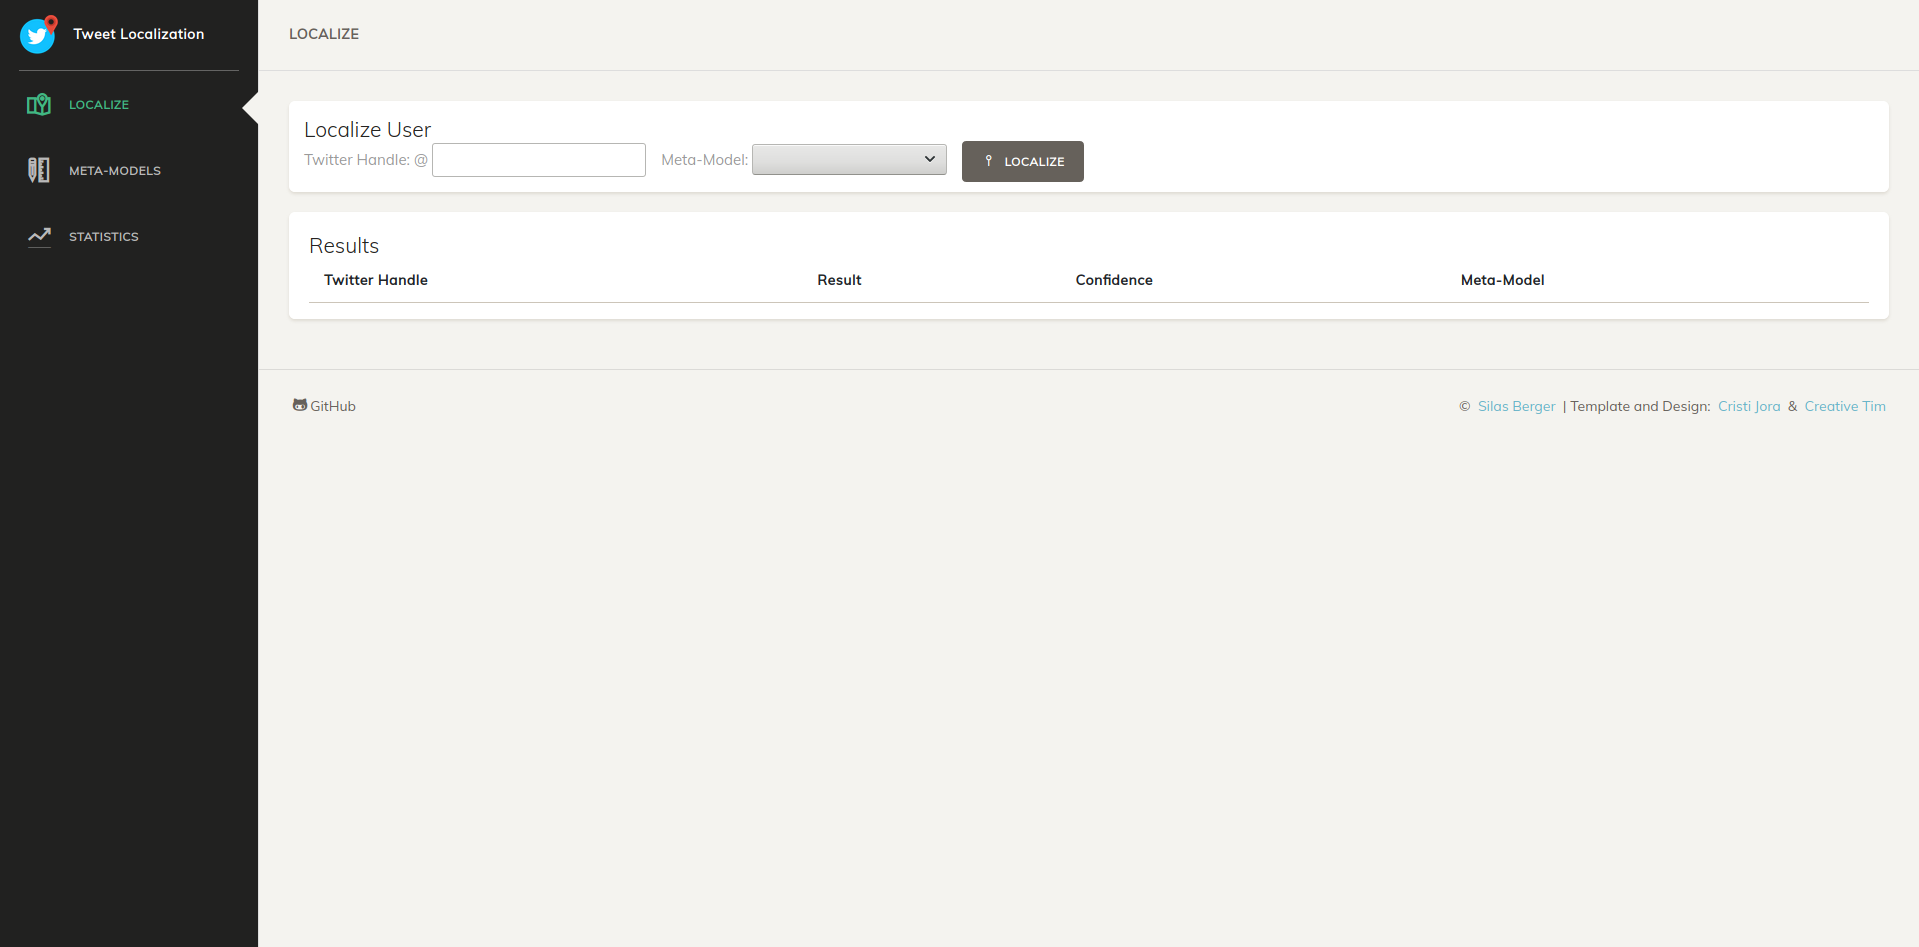
\includegraphics[scale=0.30]{localize-initial}
	\caption{Dashboard - initial localizations page}
	\label{fig:localize-initial}
\end{figure}

\begin{figure}
	\centering
	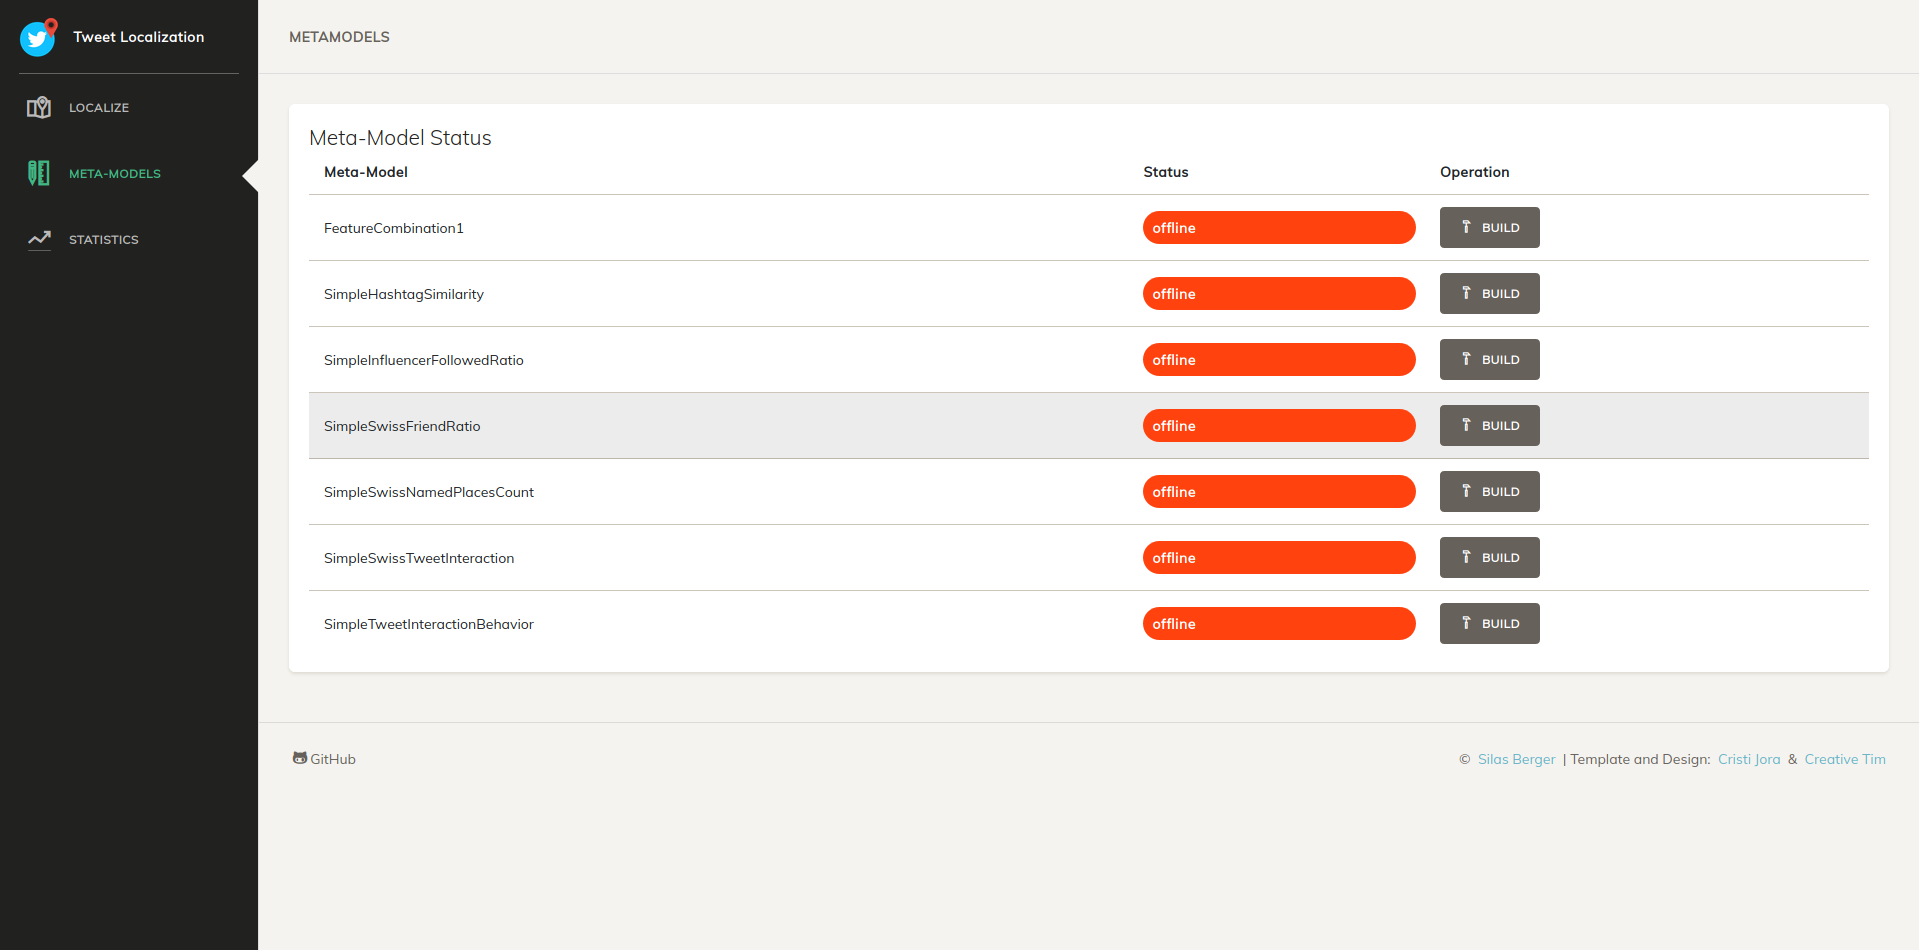
\includegraphics[scale=0.3]{metamodels-initial}
	\caption{Metamodels list, all metamodels offline}
	\label{fig:metamodels-initial}
\end{figure}

\begin{figure}
	\centering
	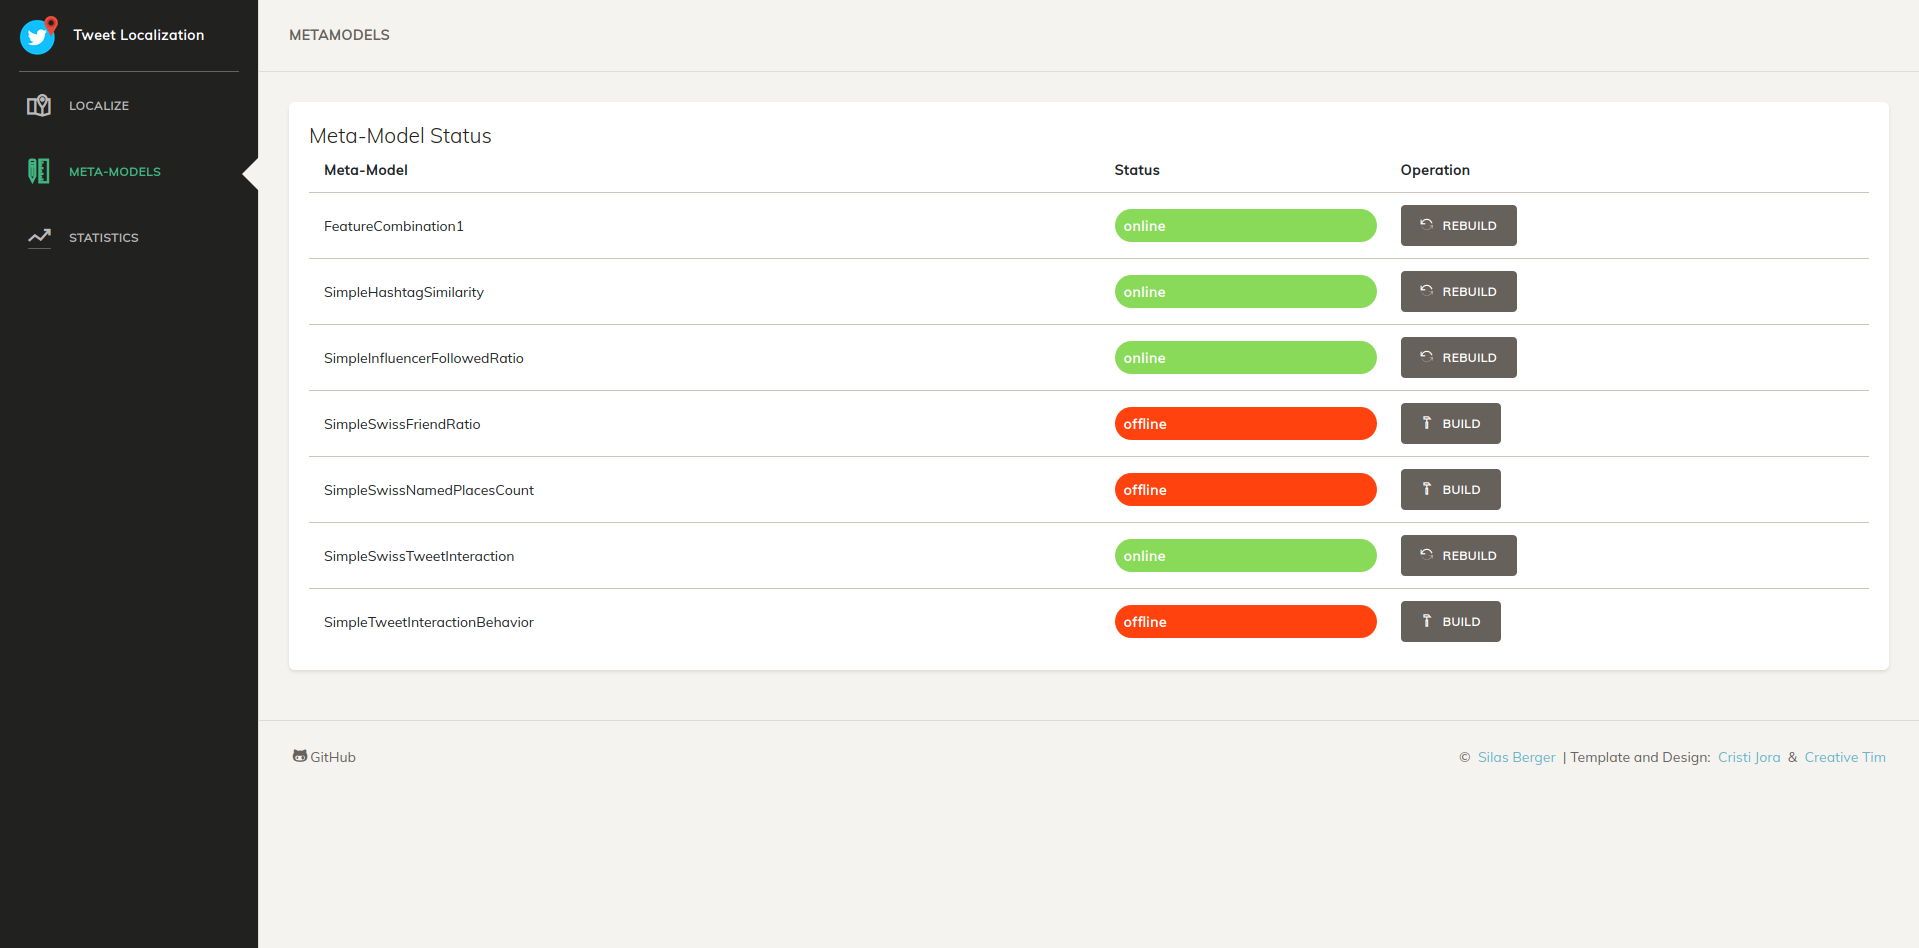
\includegraphics[scale=0.3]{metamodels-built}
	\caption{Metamodels list, multiple metamodels online}
	\label{fig:metamodels-built}
\end{figure}

\begin{figure}
	\centering
	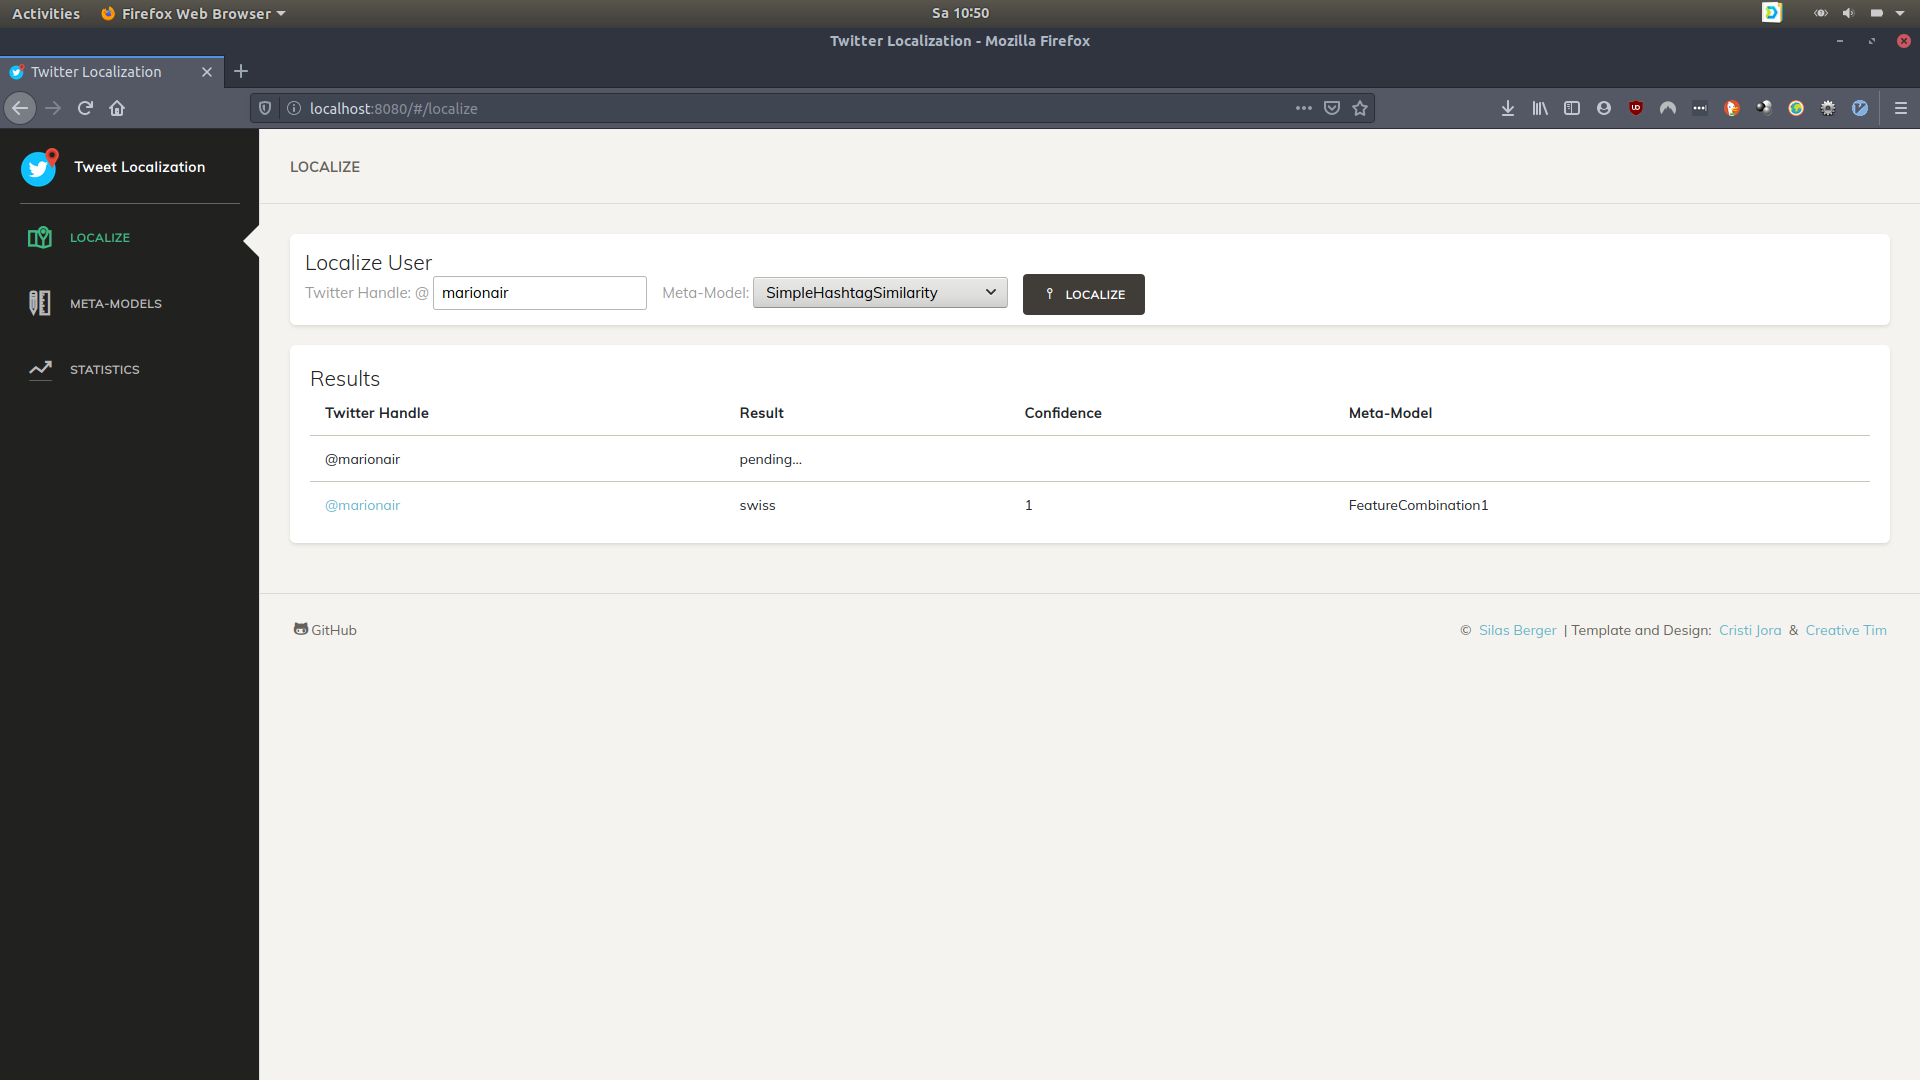
\includegraphics[scale=0.25]{localize-one-pending}
	\caption{New localization pending}
	\label{fig:localize-one-pending}
\end{figure}

\begin{figure}
	\centering
	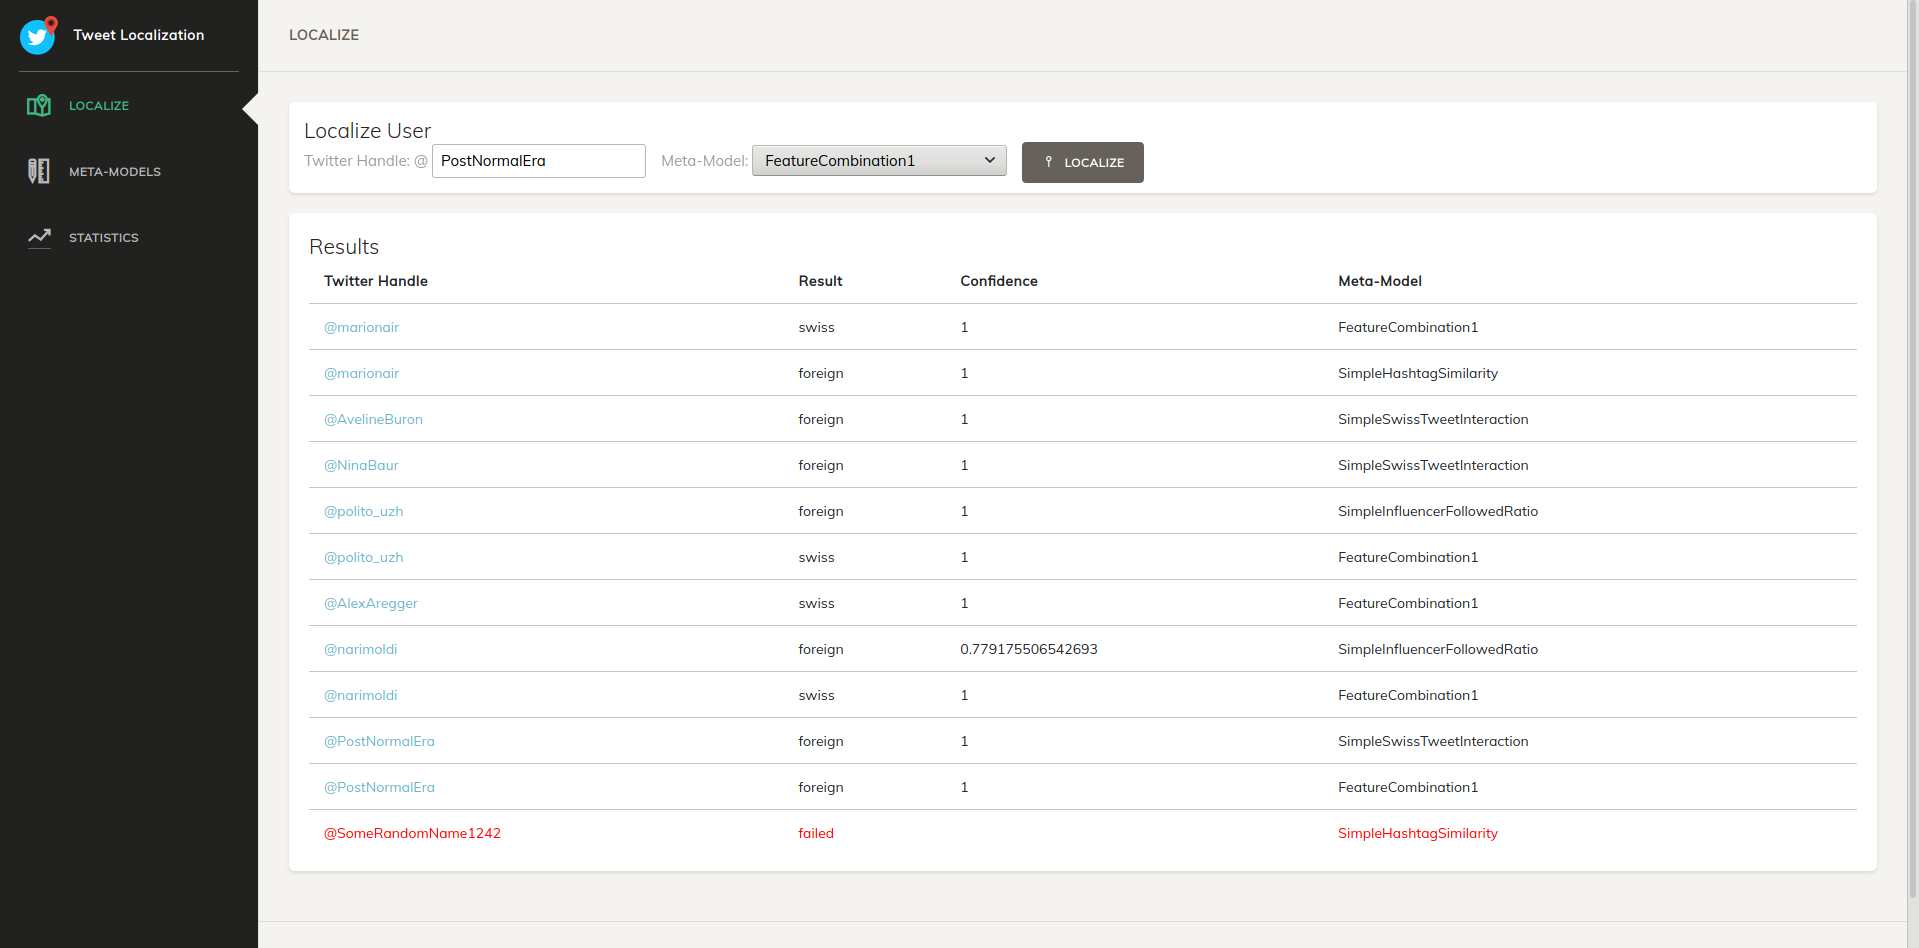
\includegraphics[scale=0.25]{localize-many-results}
	\caption{Completed and failed localizations}
	\label{fig:localize-many-results}
\end{figure}

\begin{figure}
	\centering
	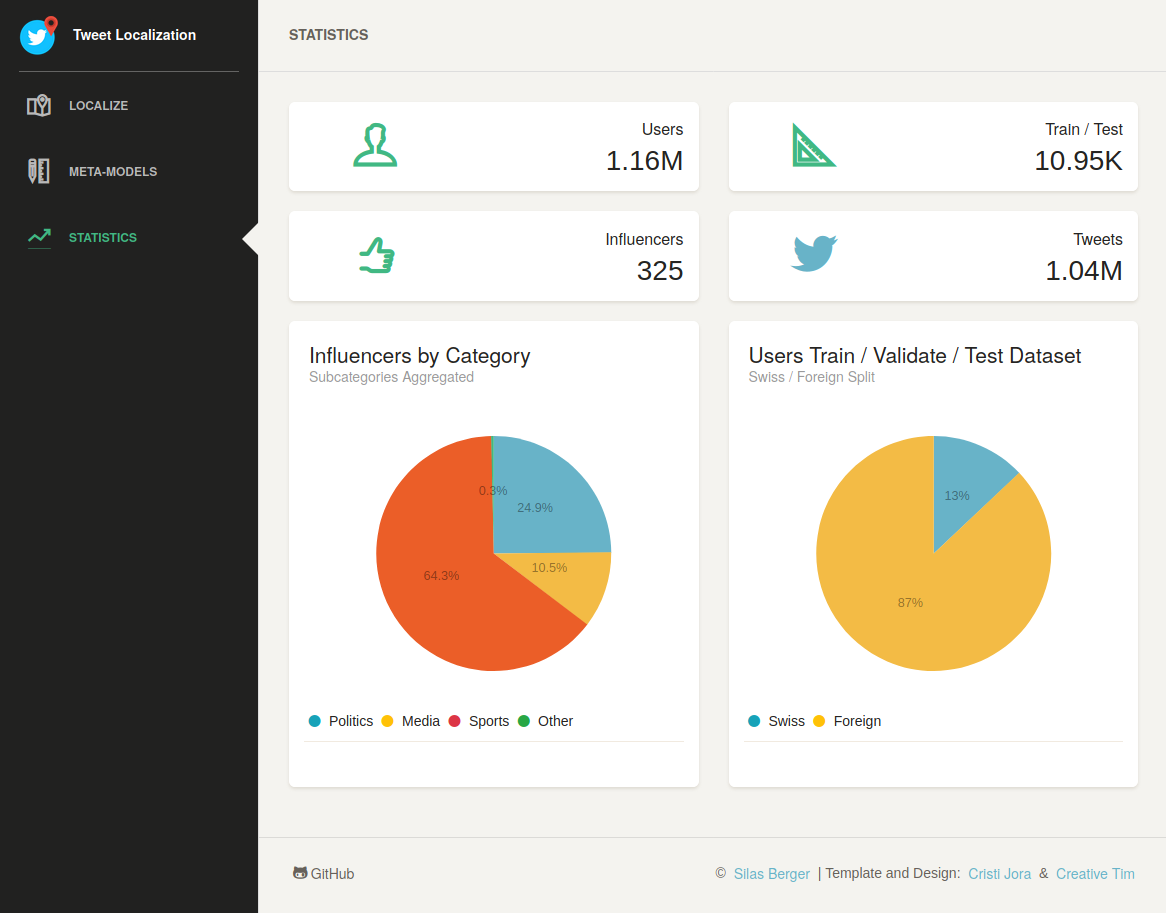
\includegraphics[scale=0.3]{statistics}
	\caption{Statistics page}
	\label{fig:statistics}
\end{figure}

\subsubsection{Implementation Details}
Each of the three pages ("Localize", "Metamodels", and "Statistics") is implemented as a Vue.js component\footnote{\href{https://vuejs.org/v2/guide/components.html}{https://vuejs.org/v2/guide/components.html}}. They all rely on a singleton object of a JavaScript class called \textbf{Context}. This object periodically queries the back end for its current metamodels status (that is, which metamodels are online, which ones are offline), as well as the current queue of pending, completed and failed localizations. The Context object caches this information, provides access to it to all the components, and raises corresponding events, whenever data has been updated. This allows the components to react to these updates and display the latest data available in the front end.

When localizing a new user, the "Localize" component uses the Context object to send a localization request to the back end. The component does not receive an immediate response to that request, as it is executed asynchronously. Once a request has been completed, the back end will move that request from its "pending" queue to either the "completed" or the "failed" queue. As soon as the Context object queries the back end for the latest localization queue the next time, all components will be updated and receive the latest results.


\section{Evaluation}
In order to evaluate the performance of our metamodels and their confidence estimates, we designed an assessment pipeline which benchmarks each meta-model on various different scores. In order to produce comparable results, we use the same train-validate-test split of the TVT set on every run. The is designed to only contain users whose location field matches a geographic location according to the GeoNames API. We therefore consider this geographic location to be our ground truth.

When the evaluator is instantiated, it is provided with an instance of a meta-model. The evaluator then builds the meta-model using the training set. Afterwards, it lets the meta-model localize each user in the test set, whereby each localization is persisted to the graph. Once all test users are localized, the evaluator collects all localization decisions made by this model instance and compares them to the ground truth, in order to establish the confusion matrix. The confusion matrix represents the numbers of true positives ($TP$), false negatives ($FN$), false positives ($FP$) and true negatives ($TN$) among all results.

Based on the confusion matrix, we assess the meta-model's performance by calculating its accuracy, precision, recall and F-measure. These measurements are defined as follows:
\begin{equation}
accuracy := \frac{TP+TN}{TP+FN+FP+TN}
\end{equation}
\begin{equation}
precision := \frac{TP}{TP+FP}
\end{equation}
\begin{equation}
recall := \frac{TP}{TP+FN}
\end{equation}
\begin{equation}
F := 2*\frac{precision * recall}{precision + recall}
\end{equation}

In addition to the meta-model's classification performance, the evaluator also assesses the quality of the provided confidence measures. It calculates the minimum, maximum and mean confidence across all correctly classified samples, and across all incorrectly classified samples. If the confidence measure is accurate, we expect to see high confidence values for correctly classified samples and low values for incorrectly classified ones. In order to provide a comparable overall score, we defined an additional Confidence Performance Index (CPI) metric. For a given set of samples, their classification (Swiss / non-Swiss) and confidence values of these classifications, the CPI is defined as follows:
\begin{equation}
\begin{split}
confidence' := 2*(confidence-0.5) \\
cpi(confidence, classif.) := \begin{cases}
    confidence, & \text{if classif. correct}.\\
    1-confidence, & \text{otherwise}.
  \end{cases} \\
CPI_{samples} := \frac{\sum cpi(confidence, classif.)}{\#samples}
\end{split}
\end{equation}

We defined this metric in a way that is closely related to the F-measure, and allows us to assess the overall performance of our confidence estimation mechanism along a single axis. This metric works based on the fact that each confidence level must lie in the $[0.5, 1]$ interval, due to the fact that all classifiers perform a binary classification. The CPI equally rewards high confidence in correct classifications and low confidence in incorrect classifications. It also equally punishes high confidence in incorrect classifications and low confidence in correct classifications. Due to these properties, the CPI solely measures the performance of a model's confidence estimate, rather than its classification performance.

\subsection{Swiss / non-Swiss Classification}
We ran each of the "Simple" metamodels against our test set containing of 100 users, balanced between Swiss and non-Swiss. The following table shows how our metamodels performed:

\begin{center}
\begin{tabular}{ |c|c|c|c|c| }
\hline
\textbf{Meta-Model} & \textbf{Accuracy} & \textbf{Precision} & \textbf{Recall} & \textbf{F} \\
\hline
Simple Swiss Tweet Interaction & \textbf{0.93} & \textbf{0.98} & \textbf{0.87} & \textbf{0.92} \\
\hline
Simple Infleuncers Followed Ratio & 0.81 & 0.97 & 0.61 & 0.75 \\
\hline
Simple Swiss Named Places & 0.81 & 0.97 & 0.61 & 0.75 \\
\hline
\hline
Simple Tweet Interaction Behavior & 0.59 & 0.55 & 0.61 & 0.58 \\
\hline
Simple Hashtag Similarity & 0.50 & 0.25 & 0.04 & 0.07 \\
\hline
\end{tabular}
\end{center}

As we can see, the top three metamodels performed rather well, resulting in a maximum accuracy of 93\% a maximum precision of 98\%, and a maximum recall of 87\%. Two out of the three features used in these top three metamodels (\textit{Swiss Tweet Interaction} and \textit{Influencers Followed Ratio}) are based on a Twitter user's relationship network. This goes to show that analyzing this network can be a good indicator to determine whether a user is Swiss or foreign. The third feature is based on analyzing the textual content of a user's Tweets and identifying named places in Switzerland. The performance of this feature suggests that this another good indicator to determine a person as Swiss.

It stands out that \textit{Influencers Followed Ratio} and \textit{Swiss Named Places} have excellent precision, however, they show mediocre recall. In case of the former, a likely reason seems to be that our list of influencers does in fact consist of people of little interest for foreign users, but they may not reflect the interests of a large enough portion of the Swiss population. Another reason could be that many might that not every user will choose to follow Twitter accounts with domestic relevance. Instead, many might choose to follow international users and companies which are in line with their interests. In the case of the latter, the results suggest that many  users either don't mention any locations and places in their Tweets. This might again be due to the fact that users may choose to Tweet about topics such as technology, people and entertainment, rather than topics which involve the mentioning of locations, such as politics or travel.

It is also noteworthy how badly the \textit{Simple Hashtag Similarity} feature performed. A possible explanation might be the fact that many of the observed hashtags, which are found in \hyperref[sec:appendix-hashtags]{Appendix B}, can be considered noise. Additionally, many of them carry little spatial locality, or are strictly tied to recent events, which may no longer be relevant in a few weeks or even days. A more promising approach might be to not compare the list of a user's hashtags to the most common hashtags found among Swiss users, but instead to define a list of words with strong spatial locality \cite{ryoo14a}. For instance, if a user is found to tweet about recent news events of global relevance, such as military operations or political decisions of global importance, this is not a good indicator of that person being Swiss or foreign. However, if said uses hashtags that specific to Switzerland, such as names of Swiss politicians or recent changes in domestic laws, they can serve as a much more reliable indicator.

As mentioned above, we used these results to develop five additional metamodels which use a combination of more than one feature. We have evaluated these metamodels using the same pipeline as for the ones above, with the following results:

\begin{center}
\begin{tabular}{ |c|c|c|c|c| }
\hline
\textbf{Meta-Model} & \textbf{Accuracy} & \textbf{Precision} & \textbf{Recall} & \textbf{F} \\
\hline
Feature Combination 1 & 0.94 & 0.93 & 0.93 & 0.93 \\
\hline
Feature Combination 2 & 0.93 & \textbf{0.95} & 0.89 & 0.92 \\
\hline
Feature Combination 3 & \textbf{0.95} & 0.94 & \textbf{0.96} & \textbf{0.95} \\
\hline
Feature Combination 4 & 0.94 & 0.93 & 0.93 & 0.93 \\
\hline
Feature Combination 5 & 0.60 & 0.56 & 0.61 & 0.58 \\
\hline
\end{tabular}
\end{center}

To compare the results of these additional metamodels, the following table contains a consolidation of the evaluation results for all metamodels we have implemented:

\begin{center}
\begin{tabular}{ |c|c|c|c|c| }
\hline
\textbf{Meta-Model} & \textbf{Accuracy} & \textbf{Precision} & \textbf{Recall} & \textbf{F} \\
\hline
Feature Combination 3 & \textbf{0.95} & 0.94 & \textbf{0.96} & \textbf{0.95} \\
\hline
Feature Combination 1 & 0.94 & 0.93 & 0.93 & 0.93 \\
\hline
Feature Combination 4 & 0.94 & 0.93 & 0.93 & 0.93 \\
\hline
Simple Swiss Tweet Interaction & 0.93 & \textbf{0.98} & 0.87 & 0.92 \\
\hline
Feature Combination 2 & 0.93 & 0.95 & 0.89 & 0.92 \\
\hline
Simple Infleuncers Followed Ratio & 0.81 & 0.97 & 0.61 & 0.75 \\
\hline
Simple Swiss Named Places & 0.81 & 0.97 & 0.61 & 0.75 \\
\hline
Simple Tweet Interaction Behavior & 0.59 & 0.55 & 0.61 & 0.58 \\
\hline
Feature Combination 5 & 0.60 & 0.56 & 0.61 & 0.58 \\
\hline
Simple Hashtag Similarity & 0.50 & 0.25 & 0.04 & 0.07 \\
\hline
\end{tabular}
\end{center}

\textit{Feature Combination 3} is a combination of the second- and third-best performing features, but shows the best overall performance. Interestingly, this metamodel performs better than combinations 1, 2 and 4, which all contain our top-performing feature, in terms of their F-measure. While we sacrifice some precision with this model, we also significantly improve on recall.

\subsection{Confidence Estimation}
We have evaluated our approach to confidence estimation on the same test set, as outlined above. The results look as follows:

\begin{center}
\begin{tabular}{ |c|c|c|c|c| }
\hline
\textbf{Meta-Model} & \textbf{Avg. Correct} & \textbf{Avg. Incorrect} & \textbf{CPI} \\
\hline
Simple Swiss Tweet Interaction & \textbf{0.99} & \textbf{0.86} & \textbf{0.93} \\
\hline
Simple Infleuncers Followed Ratio & 0.96 & 0.84 & 0.80 \\
\hline
Simple Swiss Named Places & 0.95 & 0.80 & 0.81 \\
\hline
\hline
Simple Tweet Interaction Behavior & 0.79 & \textbf{0.79} & 0.52 \\
\hline
Simple Hashtag Similarity & 1.00 & 1.00 & 0.50 \\
\hline
\end{tabular}
\end{center}

Our results show that using class membership probability as a confidence metric works rather well for our use case. While the confidence in incorrectly classified samples is fairly high, there is a significant gap between the average confidence in correctly vs. incorrectly classified ones. This is important, as it allows us to set a threshold of confidence, below which we can choose to reject a classification. This also shows in the CPI value, which rewards high confidence in correct classifications and low confidence in incorrect classifications. We also observe a relationship between the performance of a metamodel and the performance of its confidence estimation: Our three well-performing metamodels show good performance in their CPI, while the CPI is considerably lower for the worse-performing metamodels.

\section{Conclusion and Future Work}
We have discussed our problem statement and research question, the current state of the art, our theoretical and practical approach to solving this problem and achieving our goals, and we have evaluated our the results of our experiments. In this section, we will summarize our findings, draw our conclusions, and discuss how this project can be developed further, to improve in the results, and to tackle related problems.

\subsection{Conclusion}
We have implemented a full pipeline and data set for classifying Twitter users as either Swiss or non-Swiss, including five custom features and ten metamodels. To offer users a way of interacting with our system, we implemented a REST API and a dashboard-style web front end, which allows users to easily localize a Twitter user.

Creating a custom data set of Swiss Twitter users has proven to be challenging, time-consuming task. The rate limitations imposed by the Twitter API make it difficult to quickly fetch user meta-data and Tweets for a large number of users. Additionally, it was difficult to define a set of keywords that yielded a substantial number of Tweets by Swiss users. Another limitation of our data set, similar to the ones used by related projects, is the fact that we need to rely on a set of users providing their true location on their Twitter profile, as we have to trust this user-generated data as our ground truth.

As for our research question, we were able to classify Twitter users as Swiss or non-Swiss with an accuracy of up to 95\%. Unfortunately, we can not directly compare this value to any related projects, as we are not aware of any research which has previously attempted to solve the same problem. However, as we discussed in our literature review, similar projects have attempted to localize users to a specific radius, e.g. 10km. To the best of our knowledge, the best approaches have managed to correctly localize at most 60\% of users. This goes to show that, while our approach can be more limited for certain use cases, it can indeed provide significantly more reliable result in localizing a Twitter user.

Each classification in our system also produces a confidence value alongside. These confidence values have proven to be fairly reliable for our well-performing metamodels, allowing users to reasonably determine a threshold for rejecting a classification, should their use case call for such actions.

In our implementation, we decided to persist the results of our localizations to a graph database. However, this has not proven to provide any significant benefits to our development. Instead, we believe it might have been easier to persist all data to a single database, namely, MongoDB.

\subsection{Future Work}
There are are some features which we haven't implemented as part of this project, due to time constraints. One such feature is the Social Media Connection, outlined in section 4.1, which is based on the idea of attempting to link a user's Twitter profile to their presence on other social media platforms, which could then serve as a source for additional information.

Further, we think it would be worthwhile to try and approach the classification part using Artificial Neural Networks. Since they are known to require extensive amounts of training data, as well as powerful computation hardware, we decided that such an approach was out of scope for this project.

In addition to reliably classifying a user as either Swiss or non-Swiss, future work could also go towards trying to localize a Swiss user to a particular region of the country. One promising approach to this particular problem for the German-speaking part of the country could be to leverage the fact that it has many regional dialects, which aren't subject to any authoritative reference, in regards to their grammar and orthography. What words a person uses and how they spell them can potentially carry a substantional amount of information as to what region of the country they are from. In the early months of this project, we spent some time researching this topic, with the intention of focussing on Natural Language Processing for the Swiss-German language. Since there are almost no datasets available for that, we decided to try building our own, by collecting as many Swiss-German tweets as possible. However, this proved to be much more difficult than expected. Twitter doesn't recognize Swiss-German as its own language, which makes the Twitter API's language filter options unusable for such a task. Swiss-German Tweets often get recognized as being written in German, but also observed instances of them being categorized as Swedish or Dutch. One potential solution to this problem might be to leverage the results of this project, in order to collect Swiss Twitter users. We can then collect Tweets from these users and implement a custom language recognition algorithm to correctly identify their language as either Swiss-German or not Swiss-German. In the beginning of this project, we initially intended to focus on Natural Language Processing for the Swiss-German language. As for identifying a person's origin based on their choice and spelling of certain words, we see large potential in using the Sprachatlas der Deutschen Schweiz (Language Atlas of German Switzerland) \cite{sprachatlas_der_deutschen_schweiz}. Data sets based on this book can be found online\footnote{\href{http://dialektkarten.ch/index.html}{http://dialektkarten.ch/index.html}}. A promising approach to use these data seems to be to scan a user's Tweets for words listed in the Atlas and mapping these words to the regions in which they are used, with that particular spelling. The center of gravity of all points (or a cluster thereof) might be an indicator as to where the author of this particular Tweet is from.

To use our system productively, we also see some potential in improving the API and front end, such as improving responsiveness and error handling. Also, the current end point for fetching pending, completed and failed localization queries will always return the full queue. While this is fine as a proof of concept, it may lead to performance issues if the system is used in production, as every new localization query increases the amount of data that needs to be sent upon such a request. This could potentially be solved by letting the front end keep track of the latest queue item index it has received, and then only requesting items after that index from the back end. Aside from that, we think that the statistics page has potential for more interesting evaluations. For instance, users might be interested in seeing a the percentage of Twitter users localized as Swiss vs. non-Swiss so far, or visualizations of commonalities between Swiss vs. non-Swiss Twitter users, such as their most used hashtags. Finally, it could be useful to extend the API and front end to allow for administrational tasks at run time. Such tasks could include adding new training data, as well as updating our list of influencers. This is not currently supported, and users will have to manually restart the back end to perform such maintanance operations.

\clearpage
\bibliography{bibliography}
\bibliographystyle{ieeetr}

\clearpage
\appendix
\section{Tweet Search Terms}
\label{sec:appendix-searchterms}
\textbf{Swiss-specific:} bundeshaus, bundesrat, ständerat, nationalrat, sbb, palais federal, conseil federal, conseil des etats, conseil national, cff, palazzo federale, consiglio federale, consiglio degli stati, consiglio nazionale, ffs
\bigbreak
\noindent\textbf{Generic:} fussball, arbeit, stau, auto, bahn, öffentlicher verkehr, radio, song, lied, kino, film, football, travail, bouchon, voiture, train, transport public, radio, chanson, cinema, film, calcio, lavoro, ingorgo, macchina, treno, trasporto pubblico, radio, song, canzone, cinema

\section{Most Common Hashtags}
\label{sec:appendix-hashtags}
The following were the 100 most common hashtags found in the Tweets we had collected from the Swiss users in our TVT set, at the time of our experiment.
\bigbreak
\noindent filo, bzo, o, suppenhuhn, verschworungstheorie, kornfeld, verbandsmaterial, livraison, altwis, queenkong, lagerdraht, kommunikationswissenschaft, langstrassenquartier, danza, kehrsiten, lagerzeit, smoothie, trimestre, vitznau, bucheli, himmelrich, gisikon, alarm, kunstlerduo, bache, allmend, himbeeren, unterschiede, resultats, nawodh, schotterwerks, profit, direction, nachtfalter, saucisses, wisskomm, carlspitteler, hitzkirch, ernte, wasserentnahmen, tierschutzorganisation, spieler, poller, biberdamm, festessen, wassermangel, umziehenistdieholle, donnees, impressionen, buron, urteils, saisonstart, sommerbeiz, moranen, walensee, gaumen, sichtung, wander, federale, gruppentouristen, grillades, amman, chinoise, te, zahlungsmittel, zonenordnung, dollar, sommerplatzchen, printausgabe, zigarettenhersteller, salzburgerfestspiele, lucernois, sponsor, schurpf, gurtenfestival19, stadtbild, ddps, nationalhymnen, neustadt, heimweh, ambitions, kaimans, realmadridatleti, planetarium, serendipita, findlinge, videobeweis, alpenrose, dipartimento, zuzuge, rutlibund, amherd, melville, diageo, hertensteinstrasse, aufforderung, federal, abenteuer, filorosso, federspiel

\clearpage
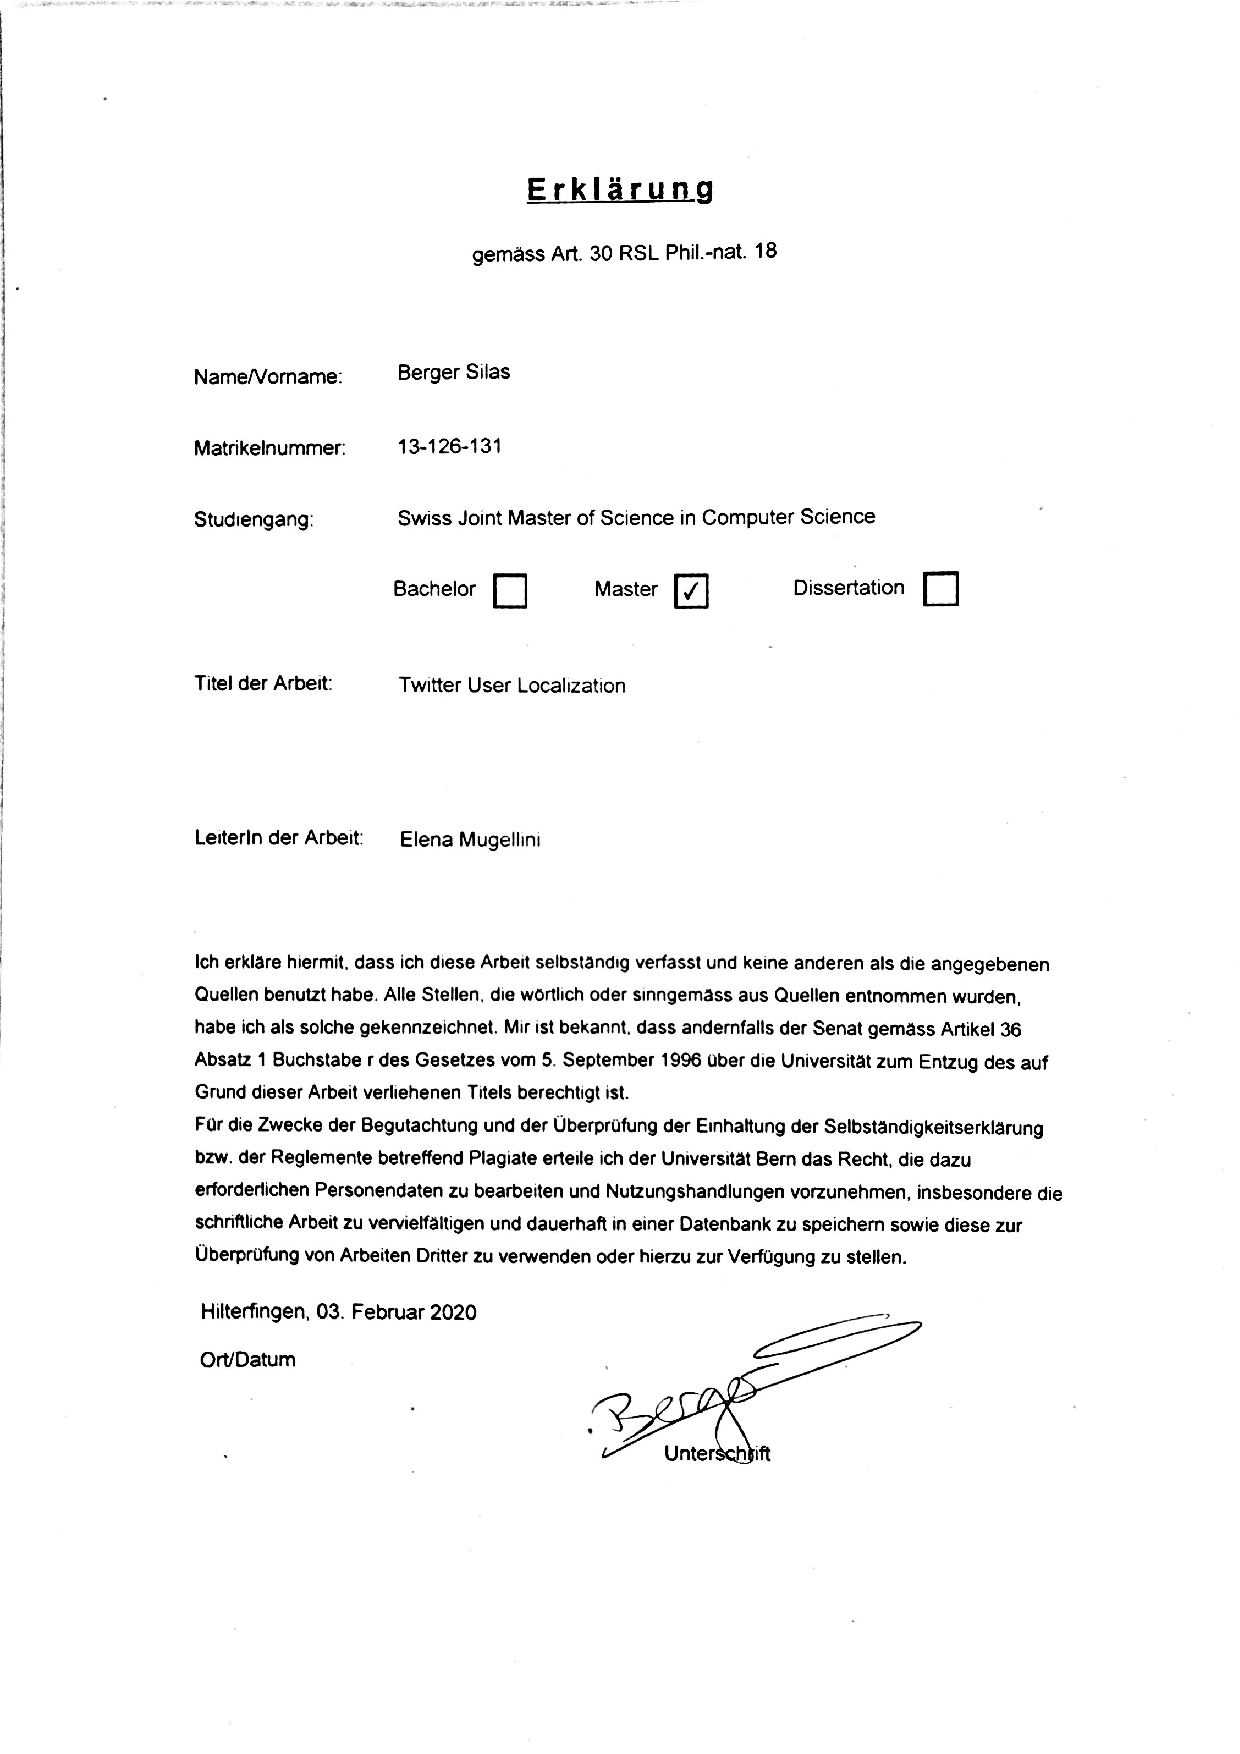
\includepdf[page={1}]{declaration}

\end{document}